% Generated by Sphinx.
\def\sphinxdocclass{report}
\documentclass[letterpaper,10pt,english]{sphinxmanual}
\usepackage[utf8]{inputenc}
\DeclareUnicodeCharacter{00A0}{\nobreakspace}
\usepackage{cmap}
\usepackage[T1]{fontenc}
\usepackage{babel}
\usepackage{times}
\usepackage[Bjarne]{fncychap}
\usepackage{longtable}
\usepackage{sphinx}
\usepackage{multirow}


\title{OpenMOOC Guide: Creating Courses}
\date{September 06, 2014}
\release{}
\author{}
\newcommand{\sphinxlogo}{}
\renewcommand{\releasename}{Release}
\makeindex

\makeatletter
\def\PYG@reset{\let\PYG@it=\relax \let\PYG@bf=\relax%
    \let\PYG@ul=\relax \let\PYG@tc=\relax%
    \let\PYG@bc=\relax \let\PYG@ff=\relax}
\def\PYG@tok#1{\csname PYG@tok@#1\endcsname}
\def\PYG@toks#1+{\ifx\relax#1\empty\else%
    \PYG@tok{#1}\expandafter\PYG@toks\fi}
\def\PYG@do#1{\PYG@bc{\PYG@tc{\PYG@ul{%
    \PYG@it{\PYG@bf{\PYG@ff{#1}}}}}}}
\def\PYG#1#2{\PYG@reset\PYG@toks#1+\relax+\PYG@do{#2}}

\expandafter\def\csname PYG@tok@gd\endcsname{\def\PYG@tc##1{\textcolor[rgb]{0.63,0.00,0.00}{##1}}}
\expandafter\def\csname PYG@tok@gu\endcsname{\let\PYG@bf=\textbf\def\PYG@tc##1{\textcolor[rgb]{0.50,0.00,0.50}{##1}}}
\expandafter\def\csname PYG@tok@gt\endcsname{\def\PYG@tc##1{\textcolor[rgb]{0.00,0.27,0.87}{##1}}}
\expandafter\def\csname PYG@tok@gs\endcsname{\let\PYG@bf=\textbf}
\expandafter\def\csname PYG@tok@gr\endcsname{\def\PYG@tc##1{\textcolor[rgb]{1.00,0.00,0.00}{##1}}}
\expandafter\def\csname PYG@tok@cm\endcsname{\let\PYG@it=\textit\def\PYG@tc##1{\textcolor[rgb]{0.25,0.50,0.56}{##1}}}
\expandafter\def\csname PYG@tok@vg\endcsname{\def\PYG@tc##1{\textcolor[rgb]{0.73,0.38,0.84}{##1}}}
\expandafter\def\csname PYG@tok@m\endcsname{\def\PYG@tc##1{\textcolor[rgb]{0.13,0.50,0.31}{##1}}}
\expandafter\def\csname PYG@tok@mh\endcsname{\def\PYG@tc##1{\textcolor[rgb]{0.13,0.50,0.31}{##1}}}
\expandafter\def\csname PYG@tok@cs\endcsname{\def\PYG@tc##1{\textcolor[rgb]{0.25,0.50,0.56}{##1}}\def\PYG@bc##1{\setlength{\fboxsep}{0pt}\colorbox[rgb]{1.00,0.94,0.94}{\strut ##1}}}
\expandafter\def\csname PYG@tok@ge\endcsname{\let\PYG@it=\textit}
\expandafter\def\csname PYG@tok@vc\endcsname{\def\PYG@tc##1{\textcolor[rgb]{0.73,0.38,0.84}{##1}}}
\expandafter\def\csname PYG@tok@il\endcsname{\def\PYG@tc##1{\textcolor[rgb]{0.13,0.50,0.31}{##1}}}
\expandafter\def\csname PYG@tok@go\endcsname{\def\PYG@tc##1{\textcolor[rgb]{0.20,0.20,0.20}{##1}}}
\expandafter\def\csname PYG@tok@cp\endcsname{\def\PYG@tc##1{\textcolor[rgb]{0.00,0.44,0.13}{##1}}}
\expandafter\def\csname PYG@tok@gi\endcsname{\def\PYG@tc##1{\textcolor[rgb]{0.00,0.63,0.00}{##1}}}
\expandafter\def\csname PYG@tok@gh\endcsname{\let\PYG@bf=\textbf\def\PYG@tc##1{\textcolor[rgb]{0.00,0.00,0.50}{##1}}}
\expandafter\def\csname PYG@tok@ni\endcsname{\let\PYG@bf=\textbf\def\PYG@tc##1{\textcolor[rgb]{0.84,0.33,0.22}{##1}}}
\expandafter\def\csname PYG@tok@nl\endcsname{\let\PYG@bf=\textbf\def\PYG@tc##1{\textcolor[rgb]{0.00,0.13,0.44}{##1}}}
\expandafter\def\csname PYG@tok@nn\endcsname{\let\PYG@bf=\textbf\def\PYG@tc##1{\textcolor[rgb]{0.05,0.52,0.71}{##1}}}
\expandafter\def\csname PYG@tok@no\endcsname{\def\PYG@tc##1{\textcolor[rgb]{0.38,0.68,0.84}{##1}}}
\expandafter\def\csname PYG@tok@na\endcsname{\def\PYG@tc##1{\textcolor[rgb]{0.25,0.44,0.63}{##1}}}
\expandafter\def\csname PYG@tok@nb\endcsname{\def\PYG@tc##1{\textcolor[rgb]{0.00,0.44,0.13}{##1}}}
\expandafter\def\csname PYG@tok@nc\endcsname{\let\PYG@bf=\textbf\def\PYG@tc##1{\textcolor[rgb]{0.05,0.52,0.71}{##1}}}
\expandafter\def\csname PYG@tok@nd\endcsname{\let\PYG@bf=\textbf\def\PYG@tc##1{\textcolor[rgb]{0.33,0.33,0.33}{##1}}}
\expandafter\def\csname PYG@tok@ne\endcsname{\def\PYG@tc##1{\textcolor[rgb]{0.00,0.44,0.13}{##1}}}
\expandafter\def\csname PYG@tok@nf\endcsname{\def\PYG@tc##1{\textcolor[rgb]{0.02,0.16,0.49}{##1}}}
\expandafter\def\csname PYG@tok@si\endcsname{\let\PYG@it=\textit\def\PYG@tc##1{\textcolor[rgb]{0.44,0.63,0.82}{##1}}}
\expandafter\def\csname PYG@tok@s2\endcsname{\def\PYG@tc##1{\textcolor[rgb]{0.25,0.44,0.63}{##1}}}
\expandafter\def\csname PYG@tok@vi\endcsname{\def\PYG@tc##1{\textcolor[rgb]{0.73,0.38,0.84}{##1}}}
\expandafter\def\csname PYG@tok@nt\endcsname{\let\PYG@bf=\textbf\def\PYG@tc##1{\textcolor[rgb]{0.02,0.16,0.45}{##1}}}
\expandafter\def\csname PYG@tok@nv\endcsname{\def\PYG@tc##1{\textcolor[rgb]{0.73,0.38,0.84}{##1}}}
\expandafter\def\csname PYG@tok@s1\endcsname{\def\PYG@tc##1{\textcolor[rgb]{0.25,0.44,0.63}{##1}}}
\expandafter\def\csname PYG@tok@gp\endcsname{\let\PYG@bf=\textbf\def\PYG@tc##1{\textcolor[rgb]{0.78,0.36,0.04}{##1}}}
\expandafter\def\csname PYG@tok@sh\endcsname{\def\PYG@tc##1{\textcolor[rgb]{0.25,0.44,0.63}{##1}}}
\expandafter\def\csname PYG@tok@ow\endcsname{\let\PYG@bf=\textbf\def\PYG@tc##1{\textcolor[rgb]{0.00,0.44,0.13}{##1}}}
\expandafter\def\csname PYG@tok@sx\endcsname{\def\PYG@tc##1{\textcolor[rgb]{0.78,0.36,0.04}{##1}}}
\expandafter\def\csname PYG@tok@bp\endcsname{\def\PYG@tc##1{\textcolor[rgb]{0.00,0.44,0.13}{##1}}}
\expandafter\def\csname PYG@tok@c1\endcsname{\let\PYG@it=\textit\def\PYG@tc##1{\textcolor[rgb]{0.25,0.50,0.56}{##1}}}
\expandafter\def\csname PYG@tok@kc\endcsname{\let\PYG@bf=\textbf\def\PYG@tc##1{\textcolor[rgb]{0.00,0.44,0.13}{##1}}}
\expandafter\def\csname PYG@tok@c\endcsname{\let\PYG@it=\textit\def\PYG@tc##1{\textcolor[rgb]{0.25,0.50,0.56}{##1}}}
\expandafter\def\csname PYG@tok@mf\endcsname{\def\PYG@tc##1{\textcolor[rgb]{0.13,0.50,0.31}{##1}}}
\expandafter\def\csname PYG@tok@err\endcsname{\def\PYG@bc##1{\setlength{\fboxsep}{0pt}\fcolorbox[rgb]{1.00,0.00,0.00}{1,1,1}{\strut ##1}}}
\expandafter\def\csname PYG@tok@kd\endcsname{\let\PYG@bf=\textbf\def\PYG@tc##1{\textcolor[rgb]{0.00,0.44,0.13}{##1}}}
\expandafter\def\csname PYG@tok@ss\endcsname{\def\PYG@tc##1{\textcolor[rgb]{0.32,0.47,0.09}{##1}}}
\expandafter\def\csname PYG@tok@sr\endcsname{\def\PYG@tc##1{\textcolor[rgb]{0.14,0.33,0.53}{##1}}}
\expandafter\def\csname PYG@tok@mo\endcsname{\def\PYG@tc##1{\textcolor[rgb]{0.13,0.50,0.31}{##1}}}
\expandafter\def\csname PYG@tok@mi\endcsname{\def\PYG@tc##1{\textcolor[rgb]{0.13,0.50,0.31}{##1}}}
\expandafter\def\csname PYG@tok@kn\endcsname{\let\PYG@bf=\textbf\def\PYG@tc##1{\textcolor[rgb]{0.00,0.44,0.13}{##1}}}
\expandafter\def\csname PYG@tok@o\endcsname{\def\PYG@tc##1{\textcolor[rgb]{0.40,0.40,0.40}{##1}}}
\expandafter\def\csname PYG@tok@kr\endcsname{\let\PYG@bf=\textbf\def\PYG@tc##1{\textcolor[rgb]{0.00,0.44,0.13}{##1}}}
\expandafter\def\csname PYG@tok@s\endcsname{\def\PYG@tc##1{\textcolor[rgb]{0.25,0.44,0.63}{##1}}}
\expandafter\def\csname PYG@tok@kp\endcsname{\def\PYG@tc##1{\textcolor[rgb]{0.00,0.44,0.13}{##1}}}
\expandafter\def\csname PYG@tok@w\endcsname{\def\PYG@tc##1{\textcolor[rgb]{0.73,0.73,0.73}{##1}}}
\expandafter\def\csname PYG@tok@kt\endcsname{\def\PYG@tc##1{\textcolor[rgb]{0.56,0.13,0.00}{##1}}}
\expandafter\def\csname PYG@tok@sc\endcsname{\def\PYG@tc##1{\textcolor[rgb]{0.25,0.44,0.63}{##1}}}
\expandafter\def\csname PYG@tok@sb\endcsname{\def\PYG@tc##1{\textcolor[rgb]{0.25,0.44,0.63}{##1}}}
\expandafter\def\csname PYG@tok@k\endcsname{\let\PYG@bf=\textbf\def\PYG@tc##1{\textcolor[rgb]{0.00,0.44,0.13}{##1}}}
\expandafter\def\csname PYG@tok@se\endcsname{\let\PYG@bf=\textbf\def\PYG@tc##1{\textcolor[rgb]{0.25,0.44,0.63}{##1}}}
\expandafter\def\csname PYG@tok@sd\endcsname{\let\PYG@it=\textit\def\PYG@tc##1{\textcolor[rgb]{0.25,0.44,0.63}{##1}}}

\def\PYGZbs{\char`\\}
\def\PYGZus{\char`\_}
\def\PYGZob{\char`\{}
\def\PYGZcb{\char`\}}
\def\PYGZca{\char`\^}
\def\PYGZam{\char`\&}
\def\PYGZlt{\char`\<}
\def\PYGZgt{\char`\>}
\def\PYGZsh{\char`\#}
\def\PYGZpc{\char`\%}
\def\PYGZdl{\char`\$}
\def\PYGZhy{\char`\-}
\def\PYGZsq{\char`\'}
\def\PYGZdq{\char`\"}
\def\PYGZti{\char`\~}
% for compatibility with earlier versions
\def\PYGZat{@}
\def\PYGZlb{[}
\def\PYGZrb{]}
\makeatother

\renewcommand\PYGZsq{\textquotesingle}

\begin{document}

\maketitle
\tableofcontents
\phantomsection\label{index::doc}


Contents:


\chapter{Permission to create a course}
\label{permission_to_create_a_course:permission-to-create-a-course}\label{permission_to_create_a_course::doc}\label{permission_to_create_a_course:openmooc-guide-creating-courses}\label{permission_to_create_a_course:id1}

\section{Overview}
\label{permission_to_create_a_course:overview}
Only administrators of the platform can do this operation. It's necessary that the administrator gives permission to create courses to an user, manually on request by email.


\section{Steps to give permission to the user as course creator}
\label{permission_to_create_a_course:steps-to-give-permission-to-the-user-as-course-creator}\begin{enumerate}
\item {} 
Click \textbf{login} to enter the platform. You must be an administrator of the platform to do the following.

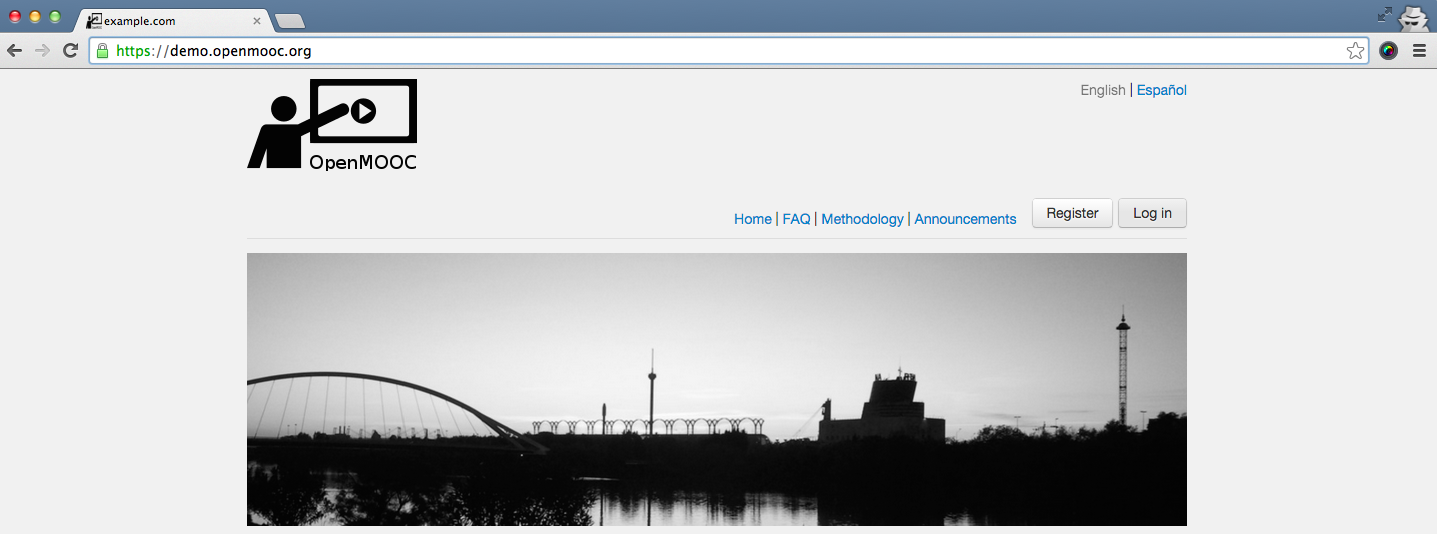
\includegraphics{0_permission_to_create_a_course-1.png}

\item {} 
Fill the \textbf{email} and \textbf{password} fields in the login form.

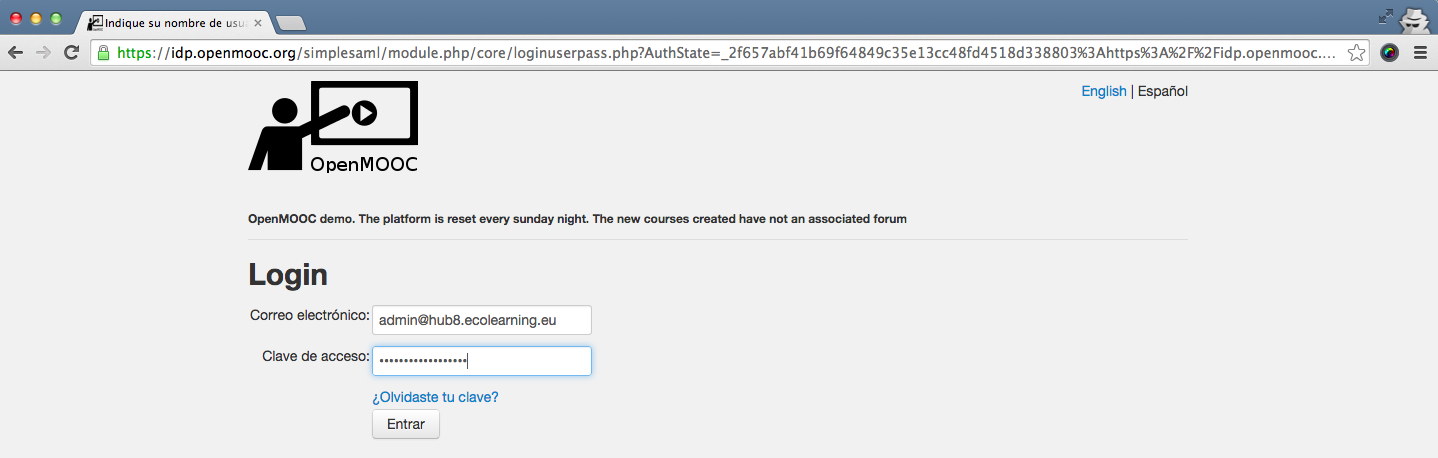
\includegraphics{0_permission_to_create_a_course-2.png}

\item {} 
When you are already logged, selected \textbf{Admin interface} in the dropdown menu you can access by clicking on the user name.

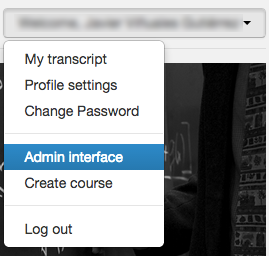
\includegraphics{0_permission_to_create_a_course-3.png}

\item {} 
You have to select \textbf{users} in the admin interface.

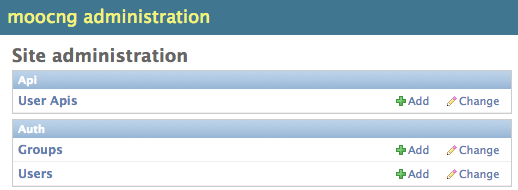
\includegraphics{0_permission_to_create_a_course-4.png}

\item {} 
Enter the name or email of the user you want to give permission to create courses in the search box

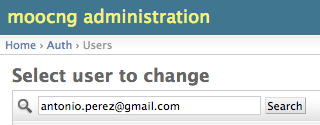
\includegraphics{0_permission_to_create_a_course-5.png}

\item {} 
Select \textbf{Staff status} to give permission to create courses to the user and click \textbf{save} on the bottom of the page.

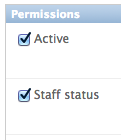
\includegraphics{0_permission_to_create_a_course-6.png}

\end{enumerate}


\chapter{Naming the course}
\label{naming_the_course::doc}\label{naming_the_course:naming-the-course}\label{naming_the_course:id1}

\section{Overview}
\label{naming_the_course:overview}
Only user with permission to crete course can do the following. It's necessary that the administrator
gives permission to create courses to an user, manually on request by email. See


\section{Steps to give to name a new course you want to create}
\label{naming_the_course:steps-to-give-to-name-a-new-course-you-want-to-create}\begin{enumerate}
\item {} 
When you are already logged, selected \textbf{Create course} in the dropdown menu you can access by clicking on the user name.

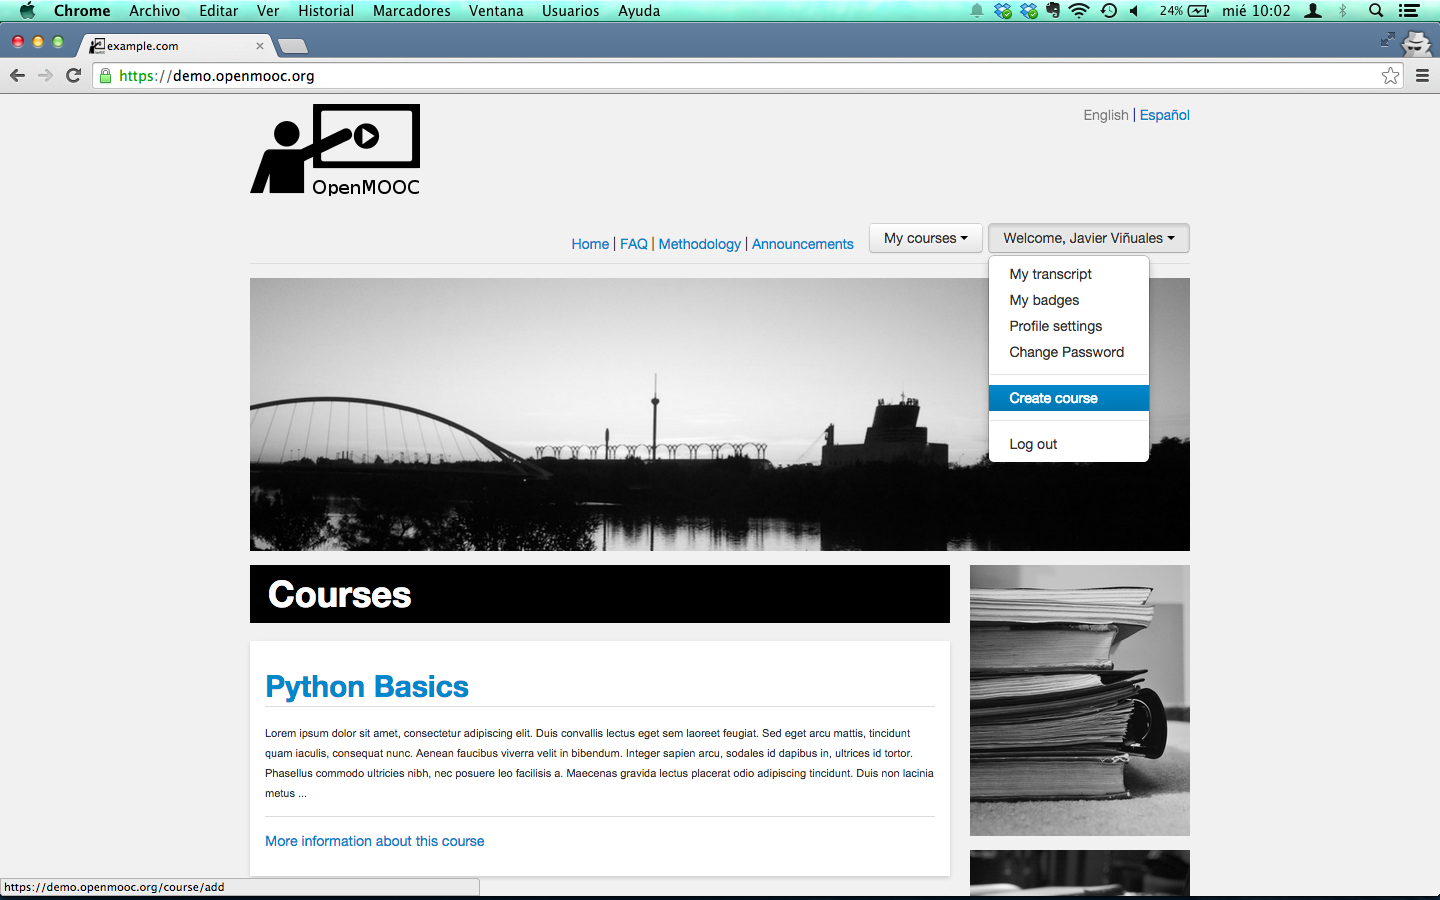
\includegraphics{1_create_course-1.png}

\item {} 
Text box you will se to enter the course name.

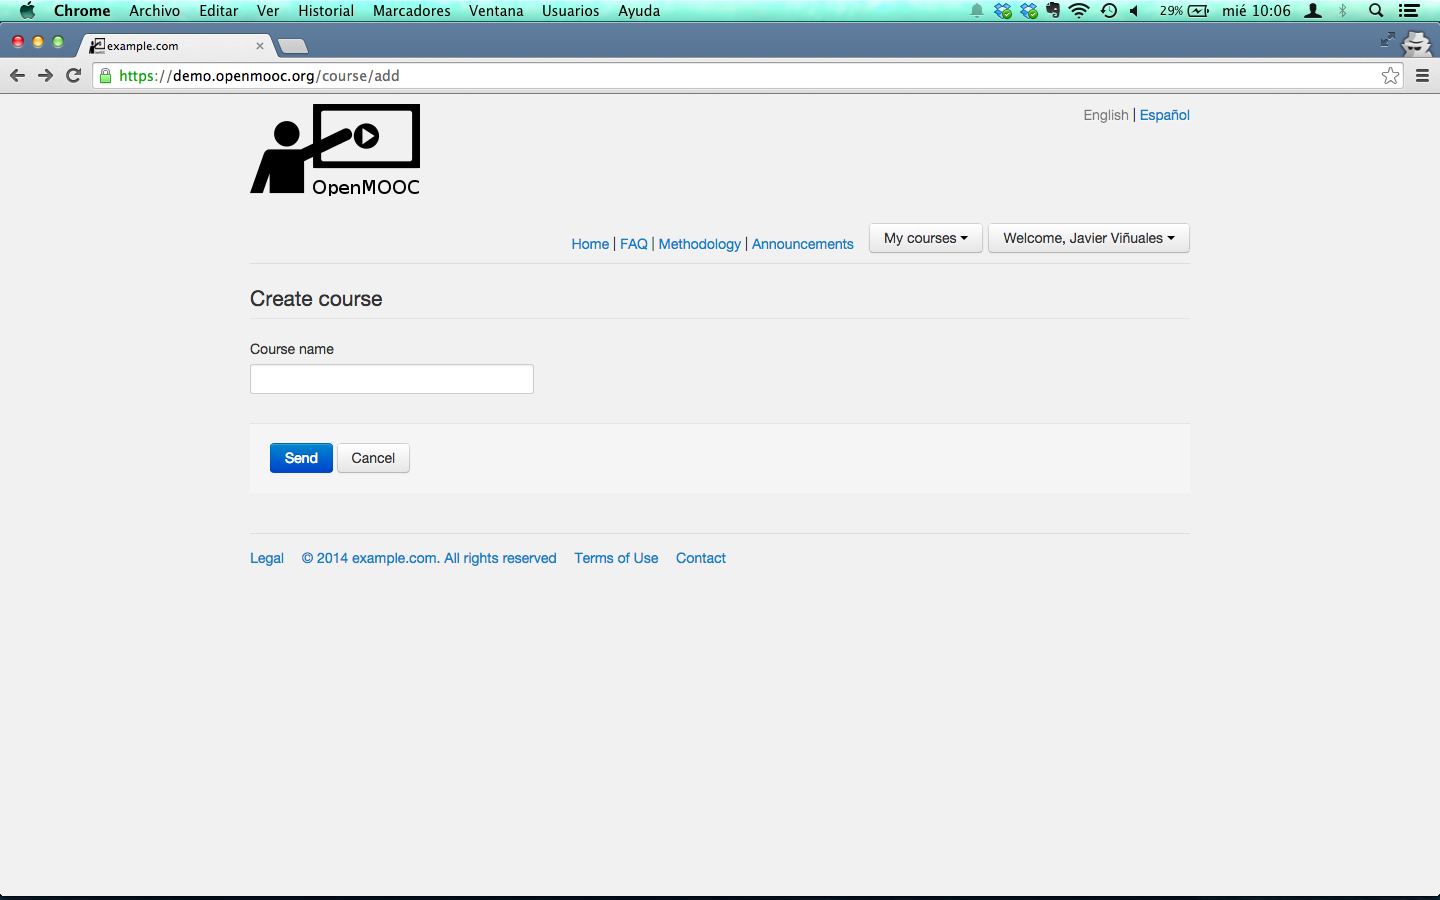
\includegraphics{2_create_course-2.png}

\item {} 
Enter the course name to create courses in the text box and click \textbf{send}.

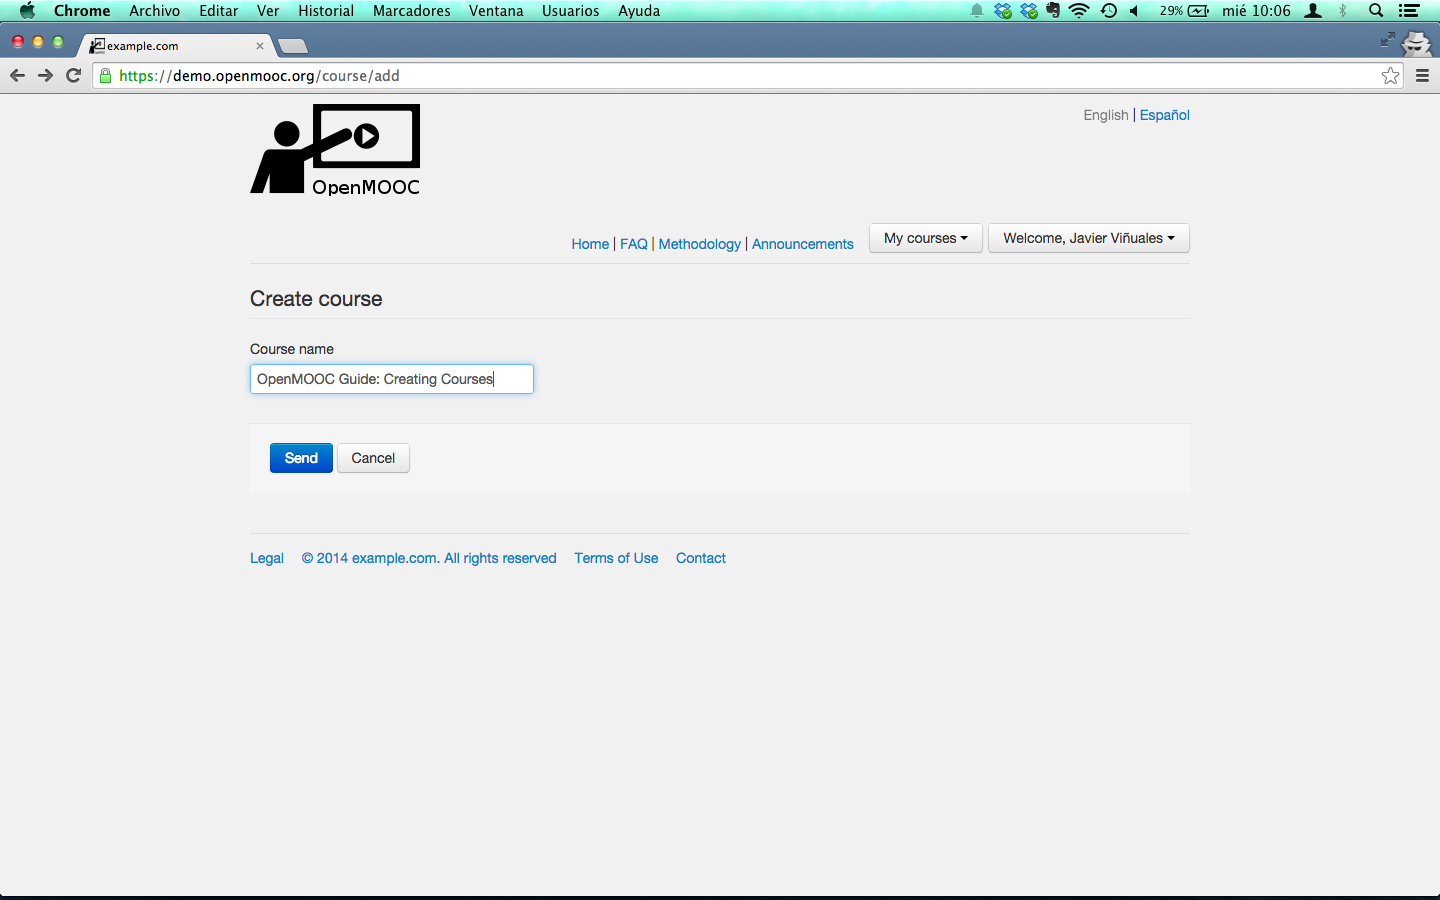
\includegraphics{3_create_course-3.png}

\end{enumerate}


\chapter{Course information}
\label{course_information:course-information}\label{course_information::doc}\label{course_information:id1}

\section{Overview}
\label{course_information:overview}
You can add a Discussion component to a unit, to pose a question related to the
Unit and give students a chance to respond and interact.


\section{Create a Discussion Component}
\label{course_information:create-a-discussion-component}\begin{enumerate}
\item {} 
Under \textbf{Add New Component}, click \textbf{Discussion}.

\item {} 
In the Discussion component that appears, click \textbf{Edit}.

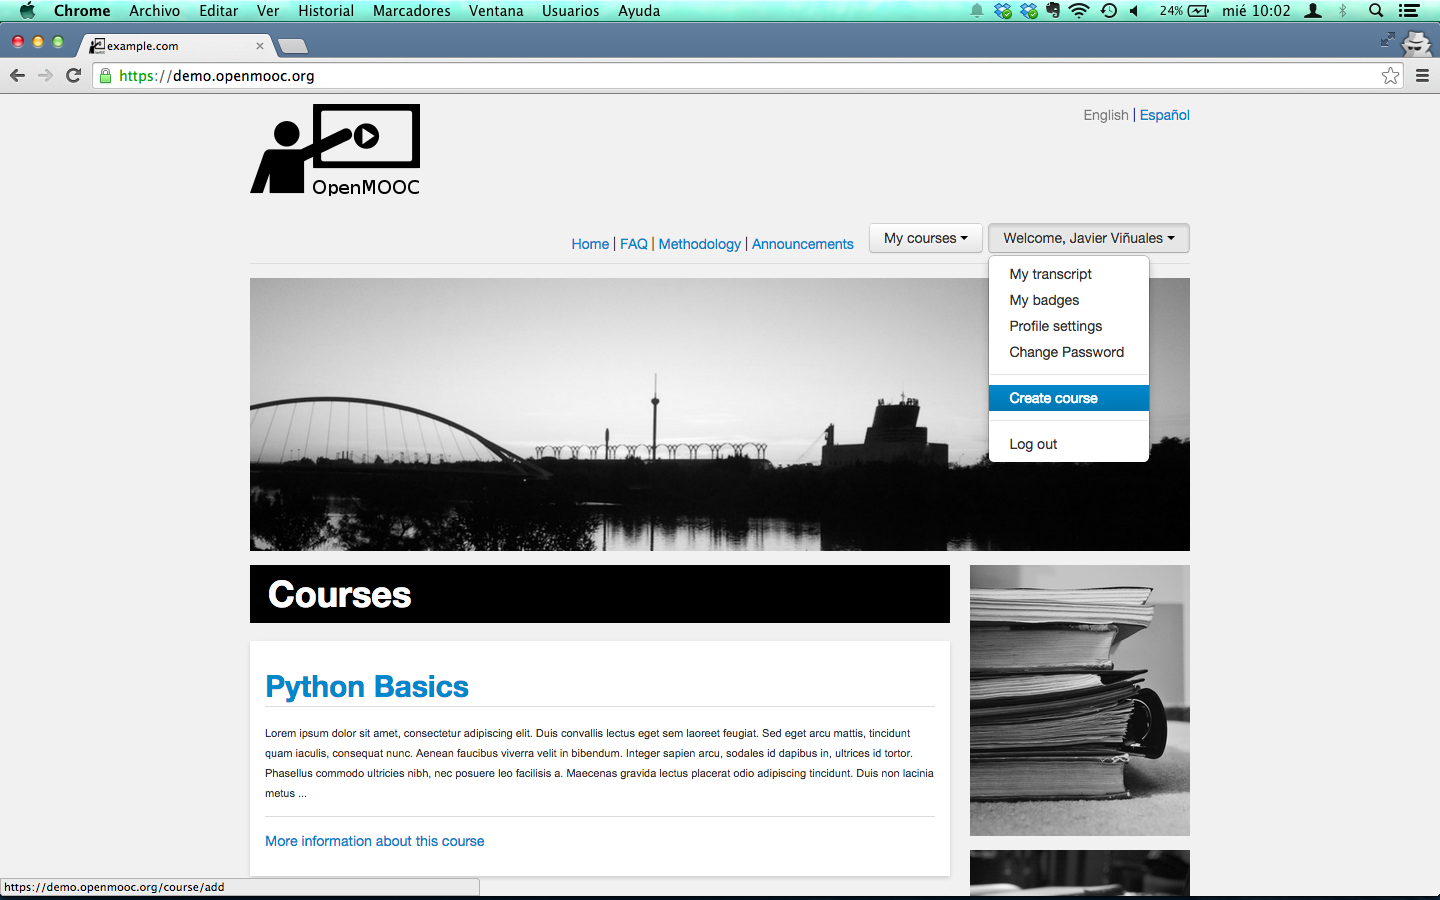
\includegraphics{1_create_course-1.png}

\item {} 
When the Discussion component editor opens, follow the guidelines in the
editor to fill in the \textbf{Category}, the optional \textbf{Display Name}, and the
\textbf{Subcategory} fields.

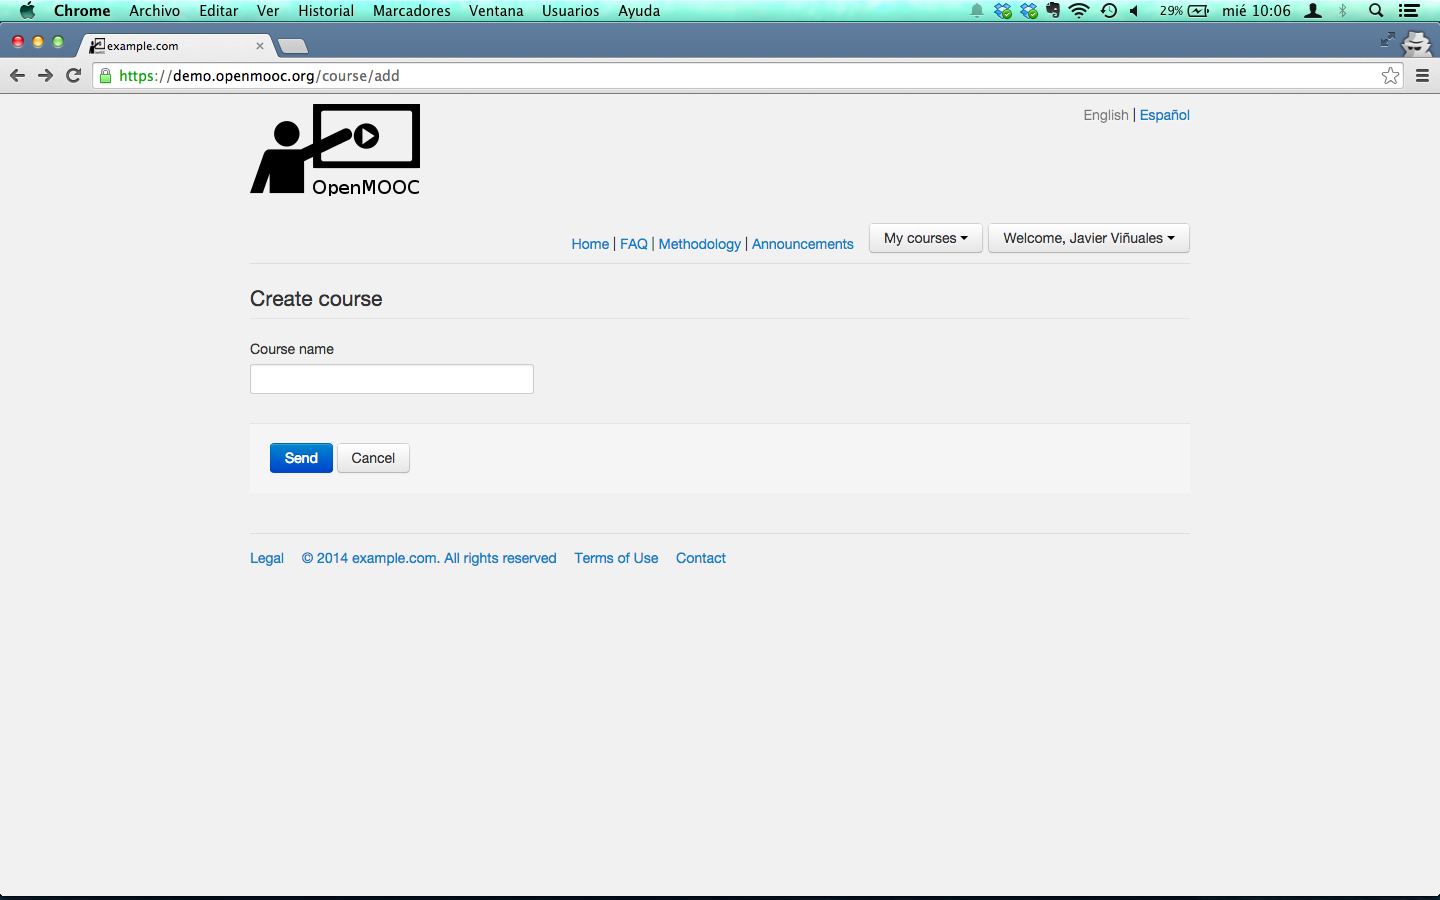
\includegraphics{2_create_course-2.png}

The value in the \textbf{Display Name} field identifies the discussion in the
course content. The values in the \textbf{Category} and \textbf{Subcategory} fields
appear in the list of discussion topics on the \textbf{Discussion} page. To
uniquely identify the discussion in your course, each \textbf{Category} /
\textbf{Subcategory} pair that you supply must be unique.

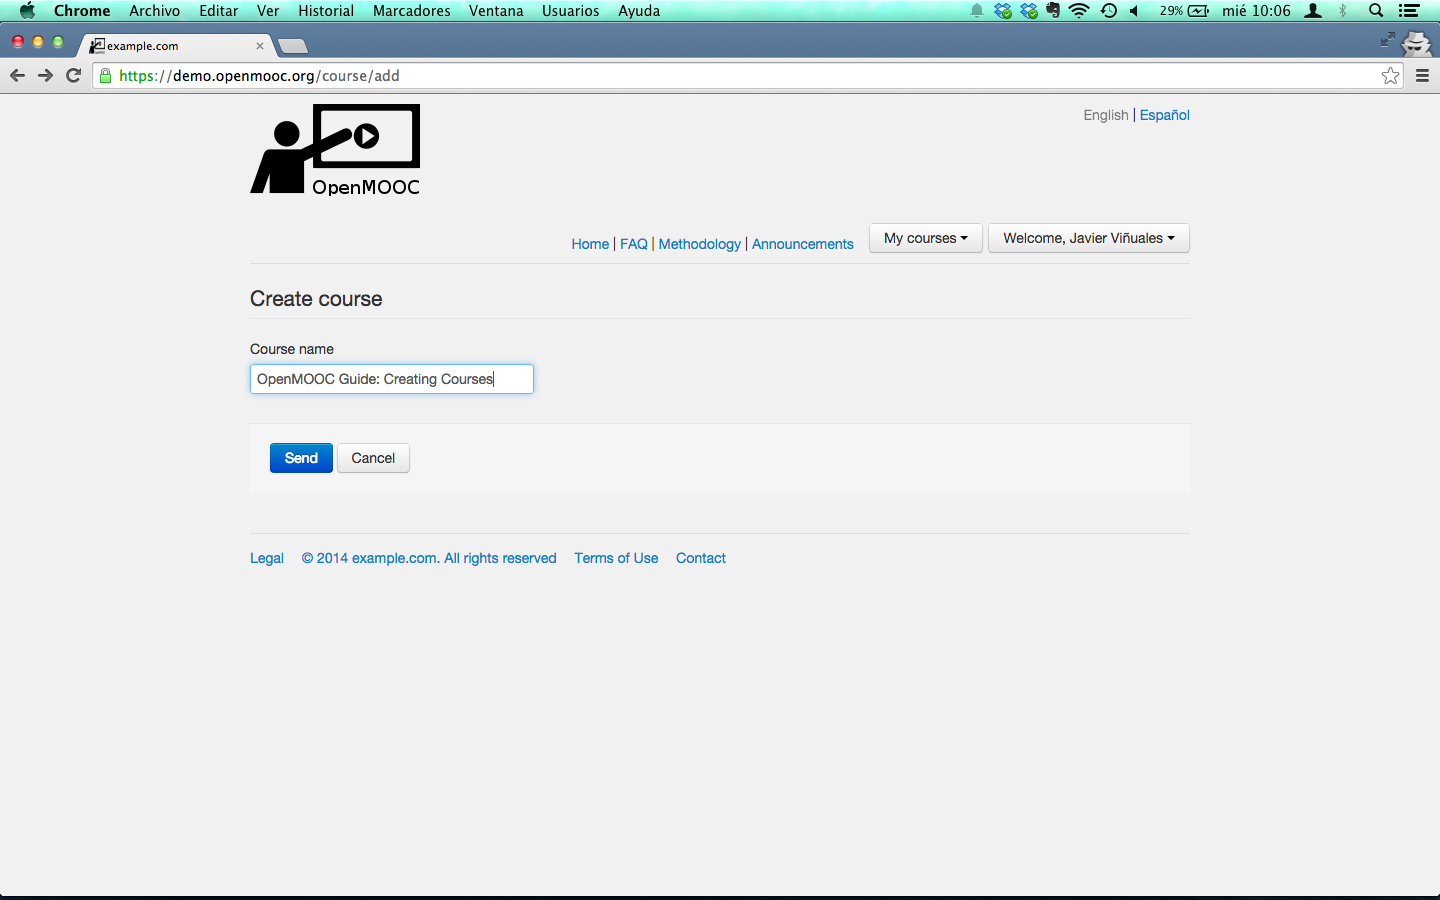
\includegraphics{3_create_course-3.png}

\end{enumerate}


\chapter{Course teachers}
\label{course_teachers:course-teachers}\label{course_teachers::doc}\label{course_teachers:id1}

\section{Overview}
\label{course_teachers:overview}
You can add a Discussion component to a unit, to pose a question related to the
Unit and give students a chance to respond and interact.


\section{Create a Discussion Component}
\label{course_teachers:create-a-discussion-component}\begin{enumerate}
\item {} 
Under \textbf{Add New Component}, click \textbf{Discussion}.

\item {} 
In the Discussion component that appears, click \textbf{Edit}.

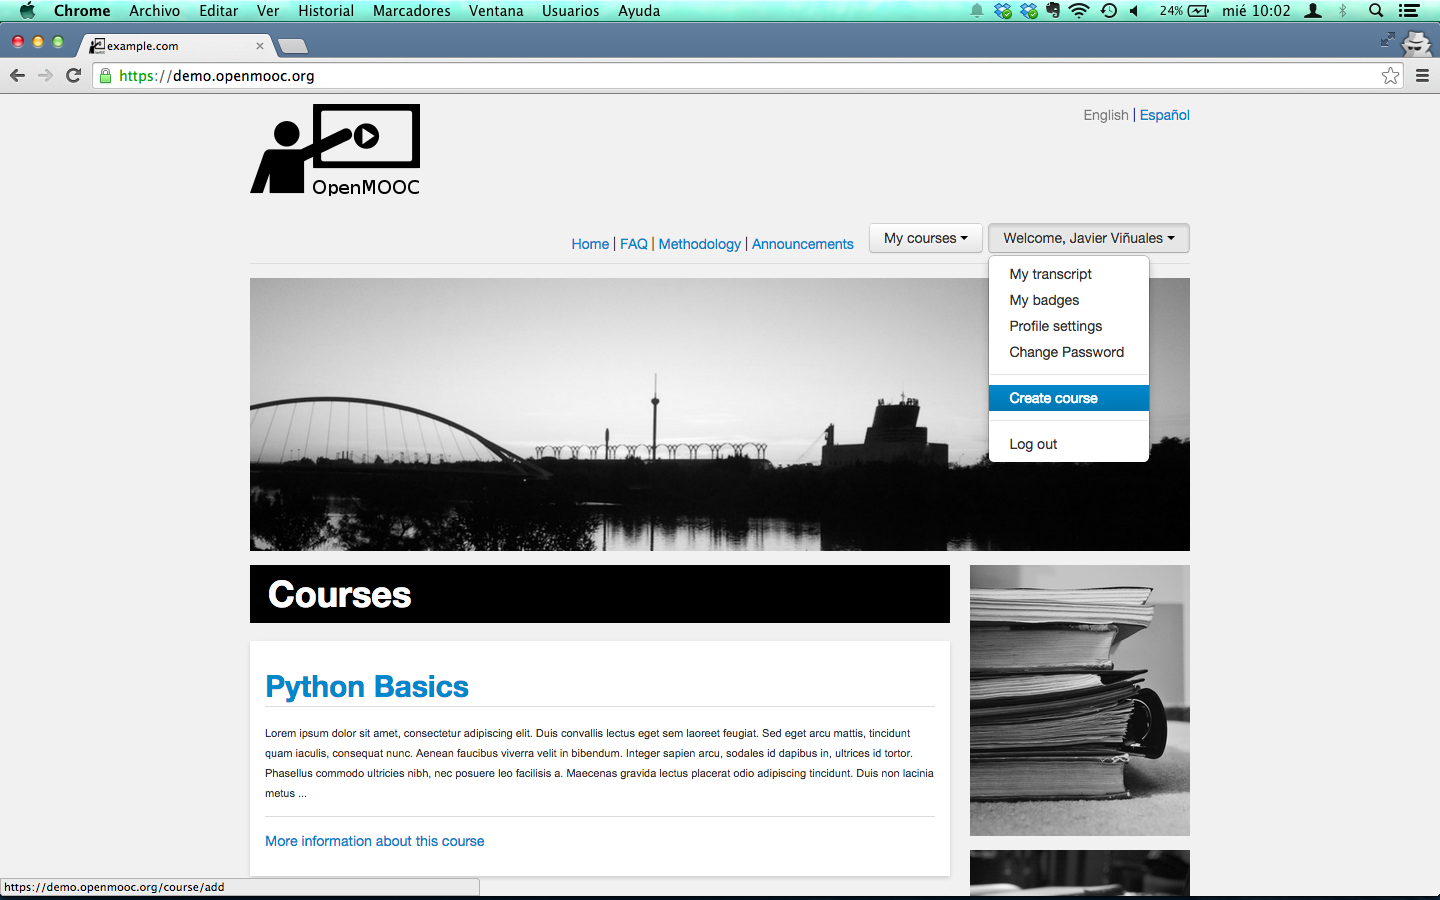
\includegraphics{1_create_course-1.png}

\item {} 
When the Discussion component editor opens, follow the guidelines in the
editor to fill in the \textbf{Category}, the optional \textbf{Display Name}, and the
\textbf{Subcategory} fields.

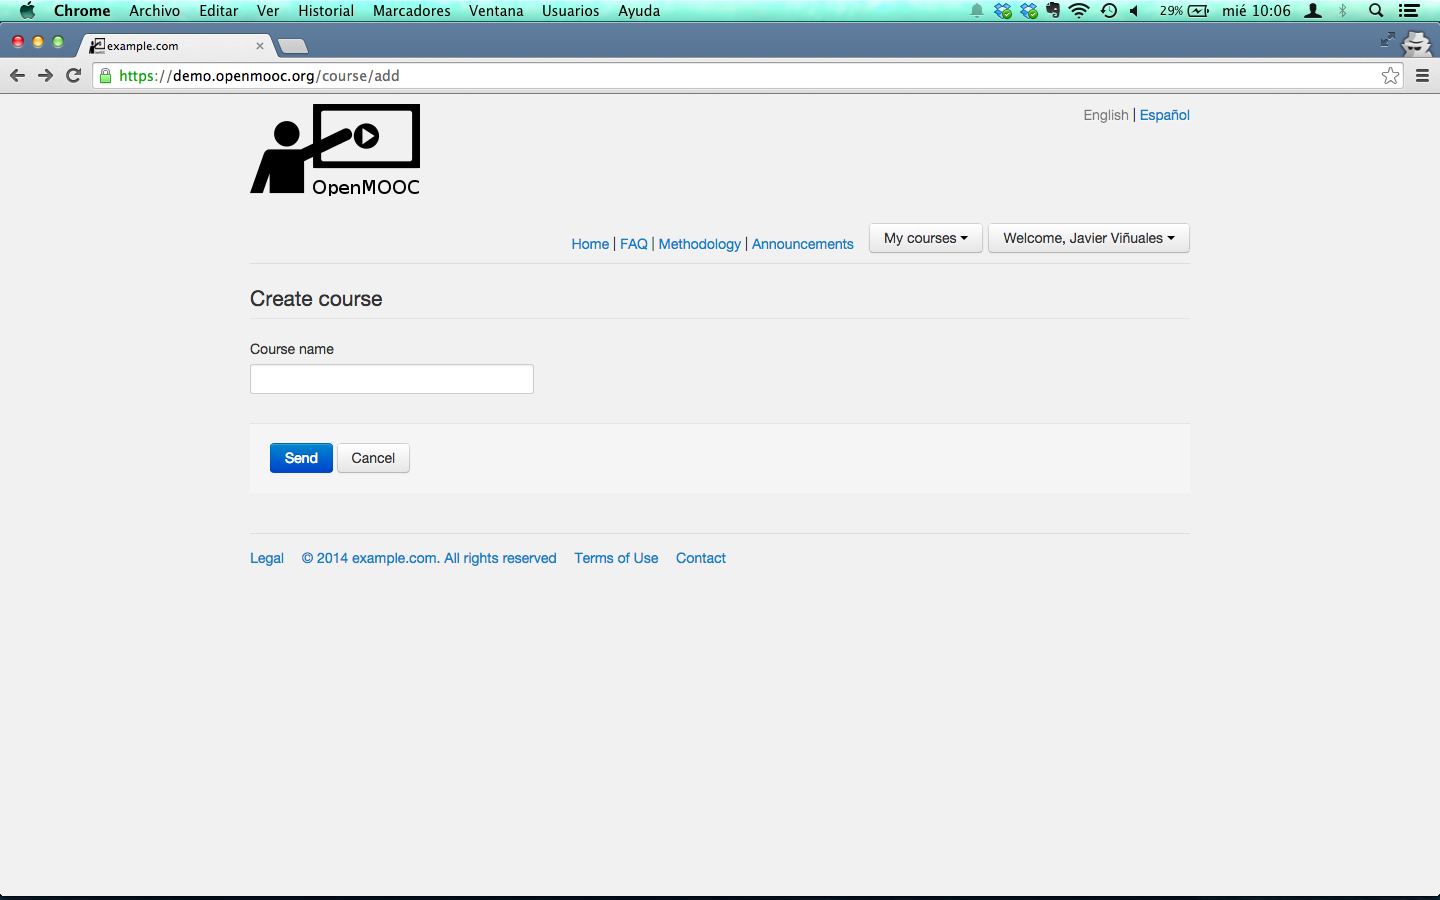
\includegraphics{2_create_course-2.png}

The value in the \textbf{Display Name} field identifies the discussion in the
course content. The values in the \textbf{Category} and \textbf{Subcategory} fields
appear in the list of discussion topics on the \textbf{Discussion} page. To
uniquely identify the discussion in your course, each \textbf{Category} /
\textbf{Subcategory} pair that you supply must be unique.

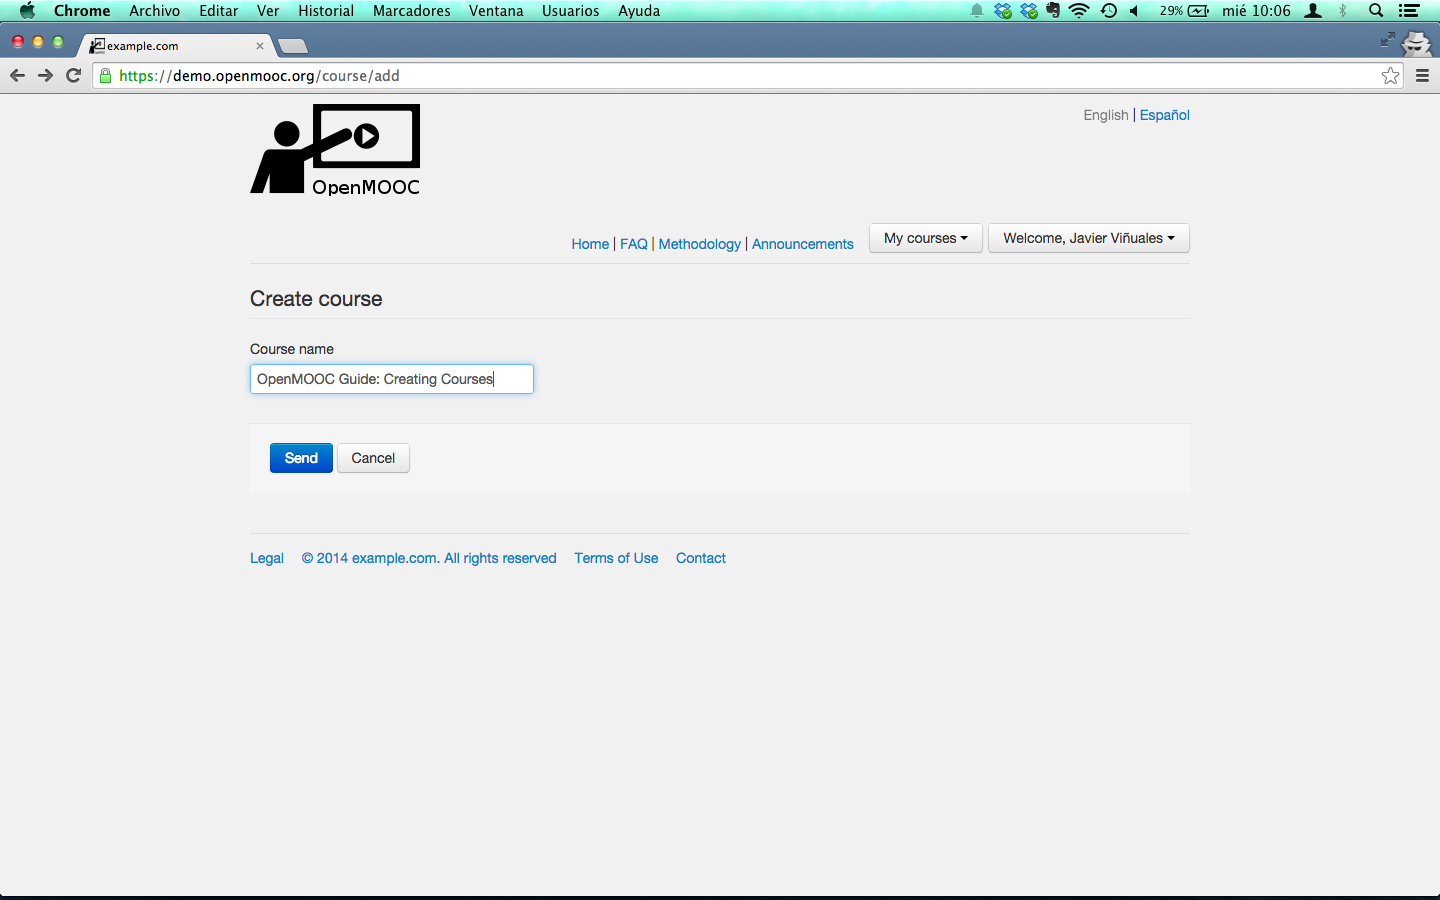
\includegraphics{3_create_course-3.png}

\end{enumerate}


\chapter{Course units}
\label{course_units:course-units}\label{course_units::doc}\label{course_units:id1}

\section{Overview}
\label{course_units:overview}
You can add a Discussion component to a unit, to pose a question related to the
Unit and give students a chance to respond and interact.


\section{Create a Discussion Component}
\label{course_units:create-a-discussion-component}\begin{enumerate}
\item {} 
Under \textbf{Add New Component}, click \textbf{Discussion}.

\item {} 
In the Discussion component that appears, click \textbf{Edit}.

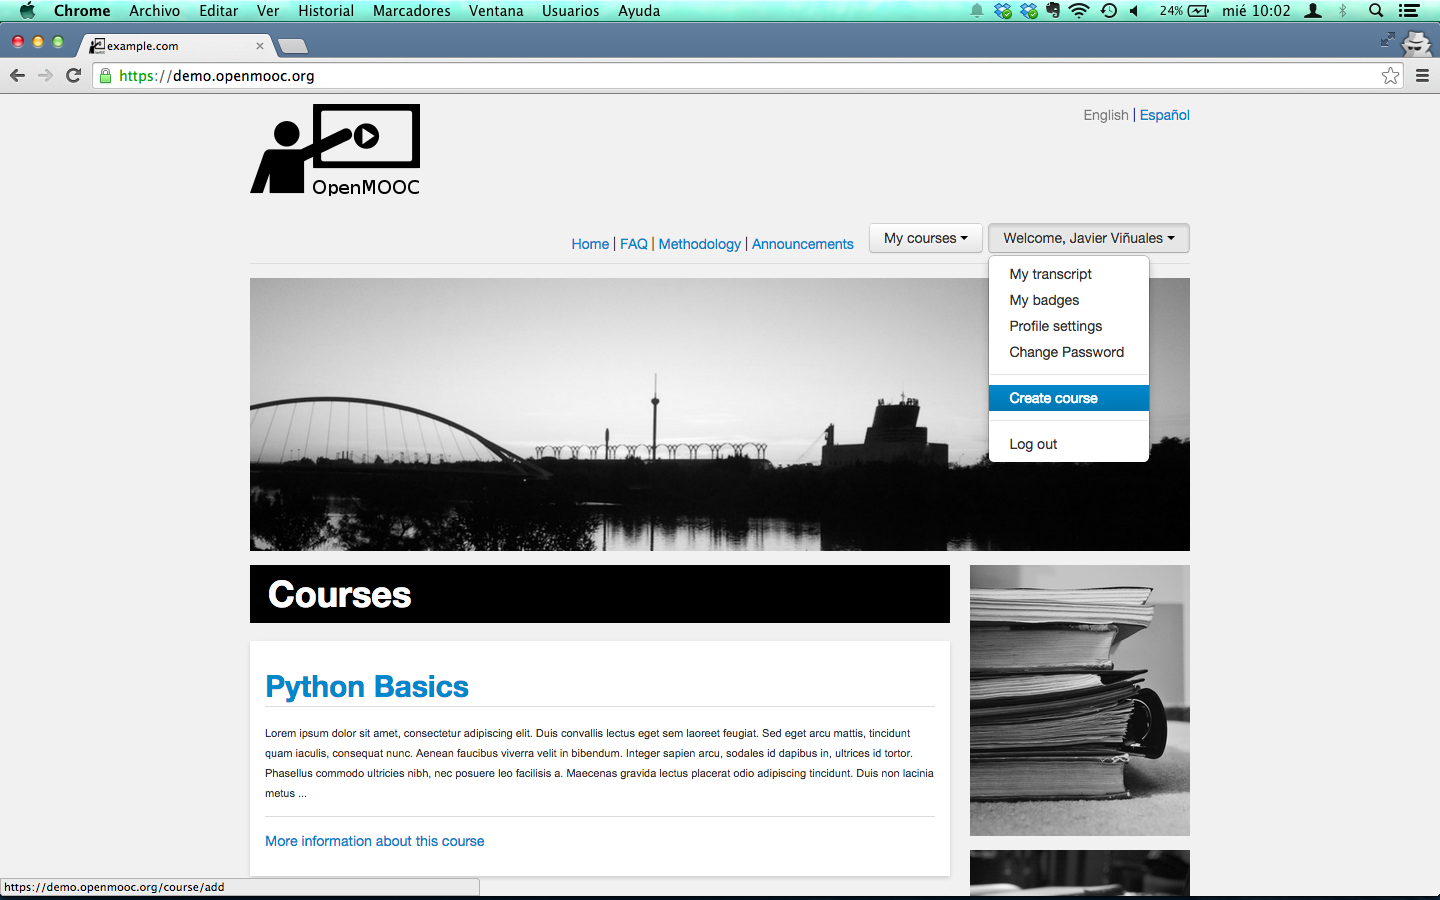
\includegraphics{1_create_course-1.png}

\item {} 
When the Discussion component editor opens, follow the guidelines in the
editor to fill in the \textbf{Category}, the optional \textbf{Display Name}, and the
\textbf{Subcategory} fields.

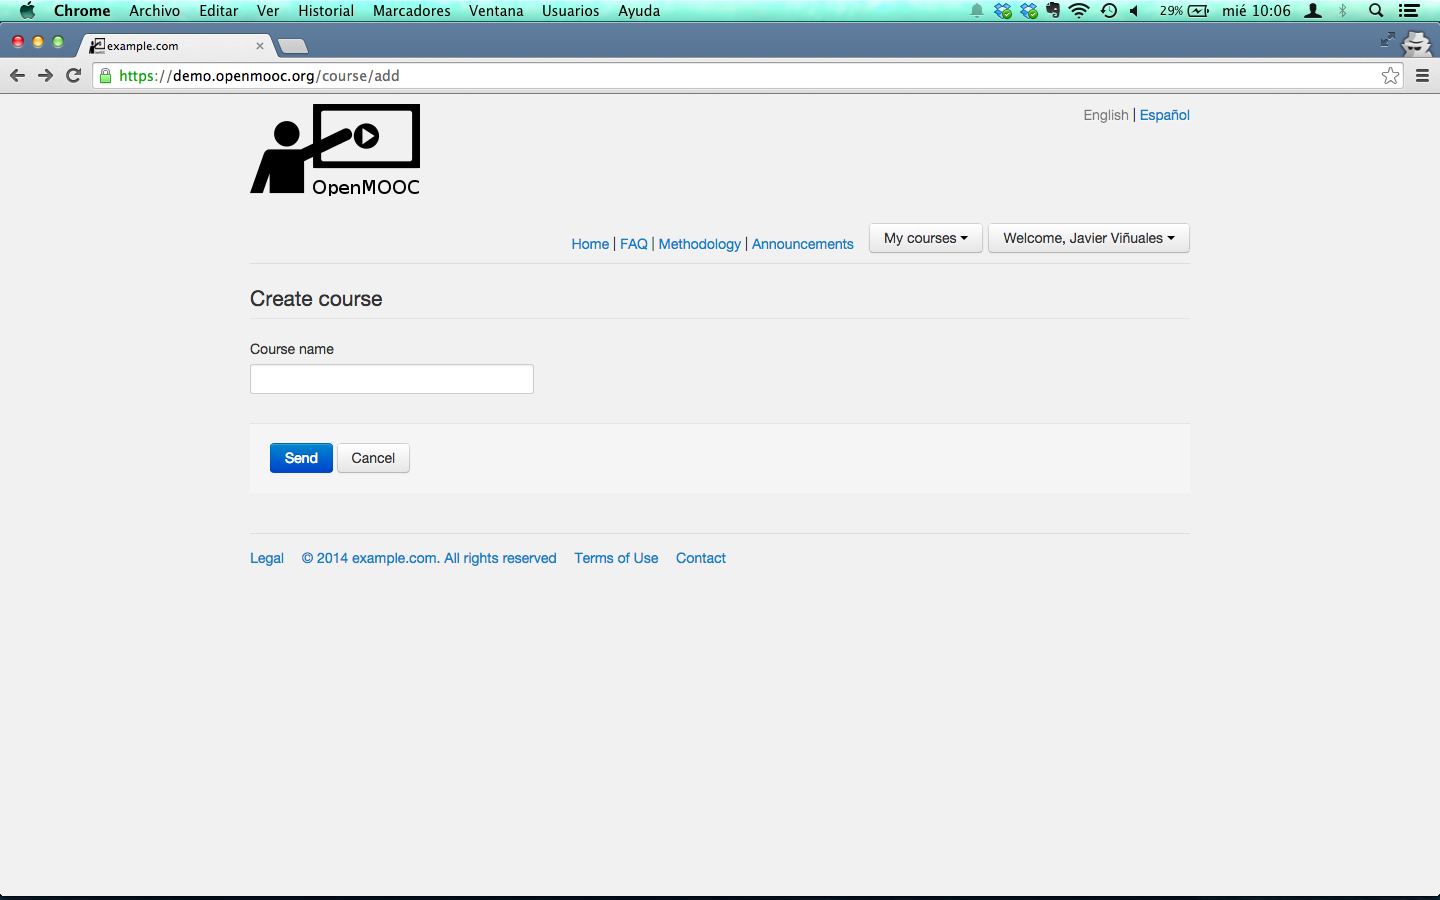
\includegraphics{2_create_course-2.png}

The value in the \textbf{Display Name} field identifies the discussion in the
course content. The values in the \textbf{Category} and \textbf{Subcategory} fields
appear in the list of discussion topics on the \textbf{Discussion} page. To
uniquely identify the discussion in your course, each \textbf{Category} /
\textbf{Subcategory} pair that you supply must be unique.

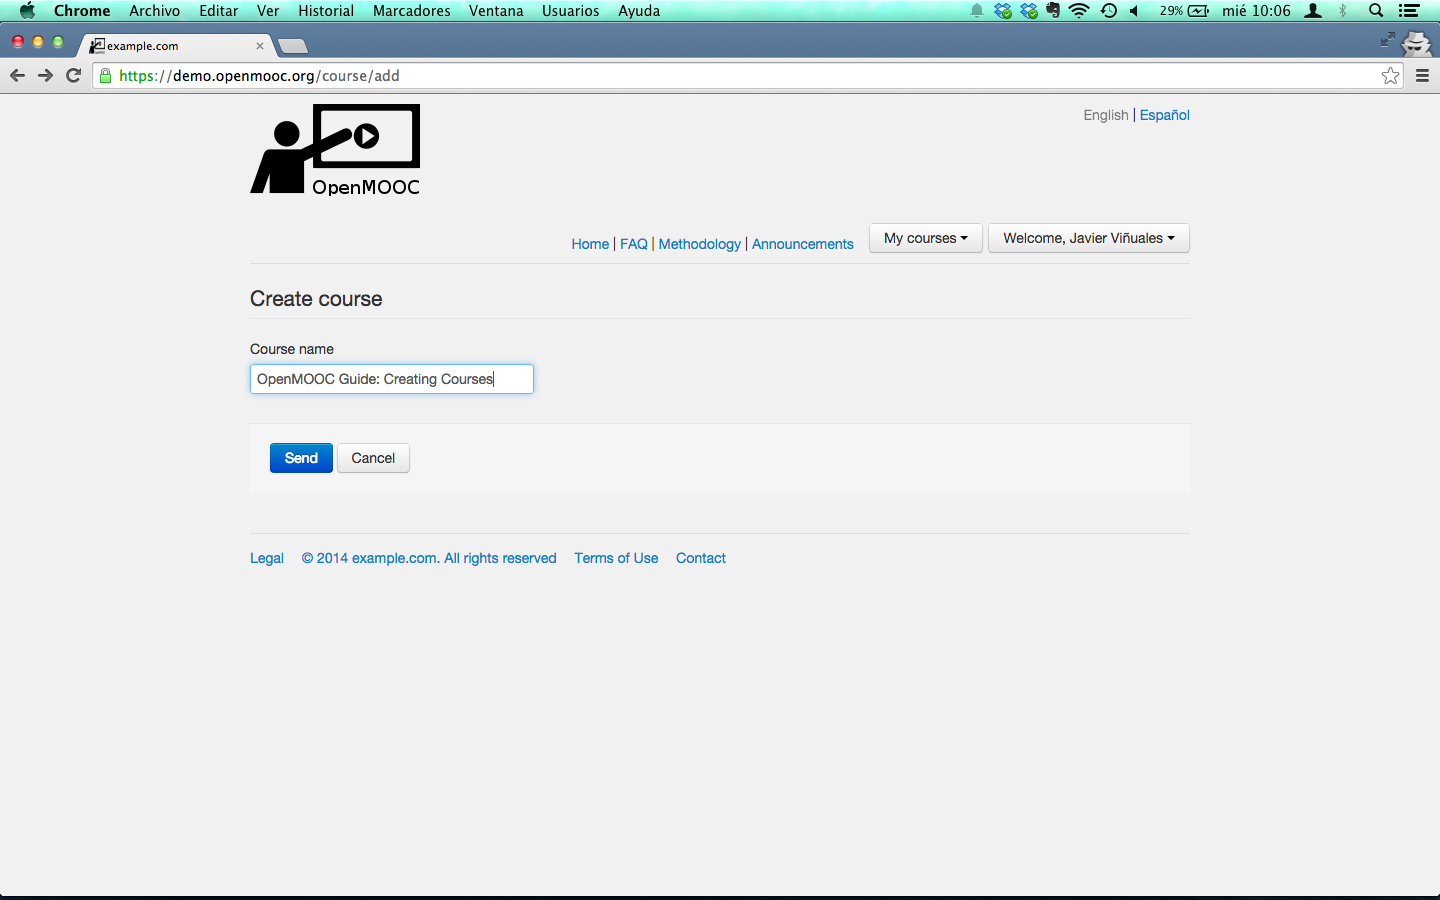
\includegraphics{3_create_course-3.png}

\end{enumerate}


\chapter{Categories}
\label{categories::doc}\label{categories:categories}\label{categories:id1}

\section{Overview}
\label{categories:overview}
You can add a Discussion component to a unit, to pose a question related to the
Unit and give students a chance to respond and interact.


\section{Create a Discussion Component}
\label{categories:create-a-discussion-component}\begin{enumerate}
\item {} 
Under \textbf{Add New Component}, click \textbf{Discussion}.

\item {} 
In the Discussion component that appears, click \textbf{Edit}.

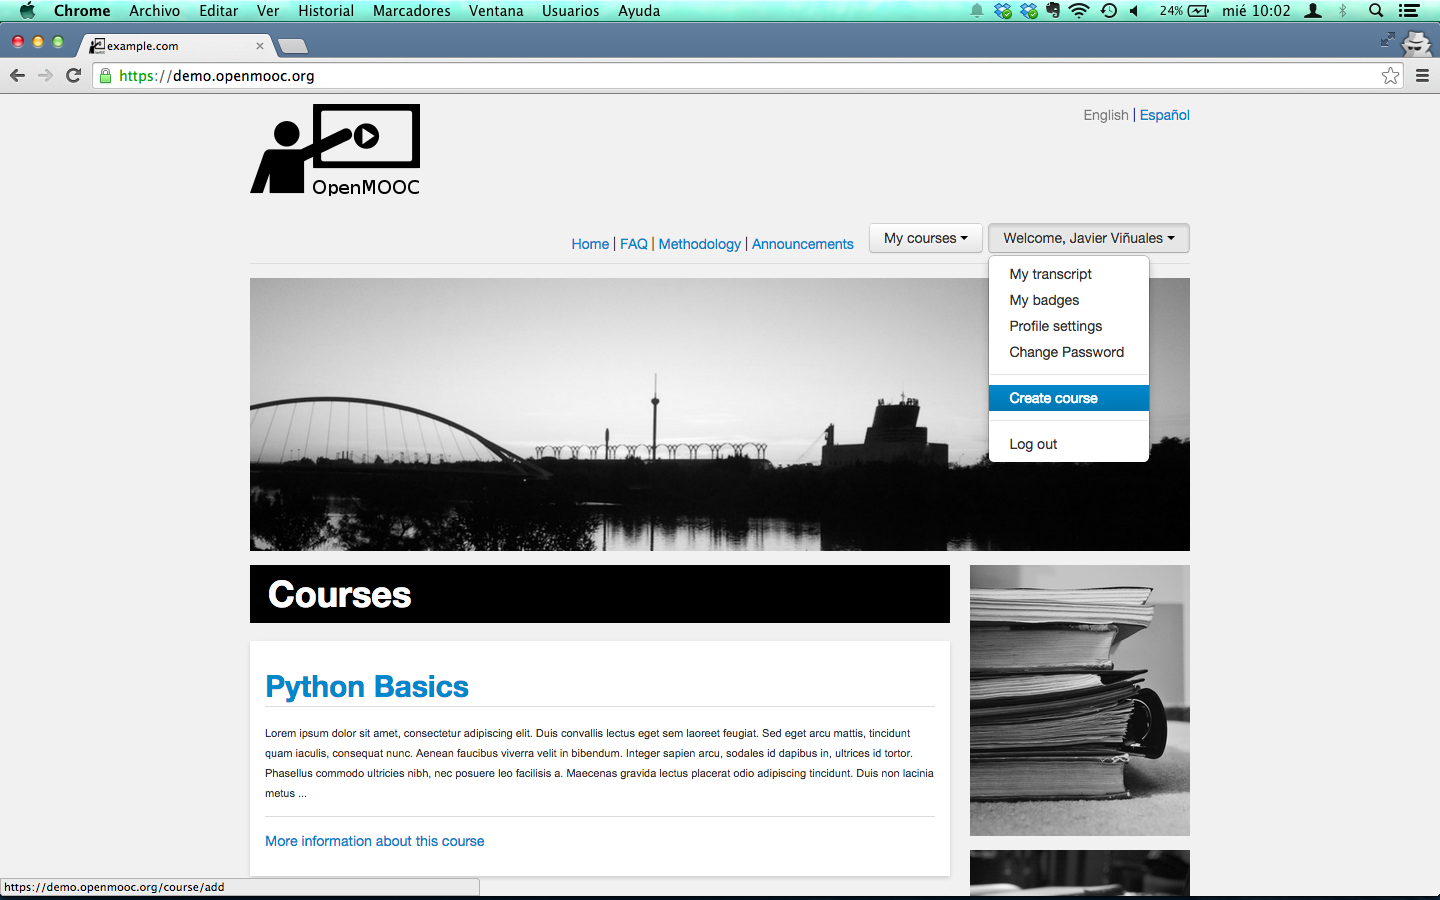
\includegraphics{1_create_course-1.png}

\item {} 
When the Discussion component editor opens, follow the guidelines in the
editor to fill in the \textbf{Category}, the optional \textbf{Display Name}, and the
\textbf{Subcategory} fields.

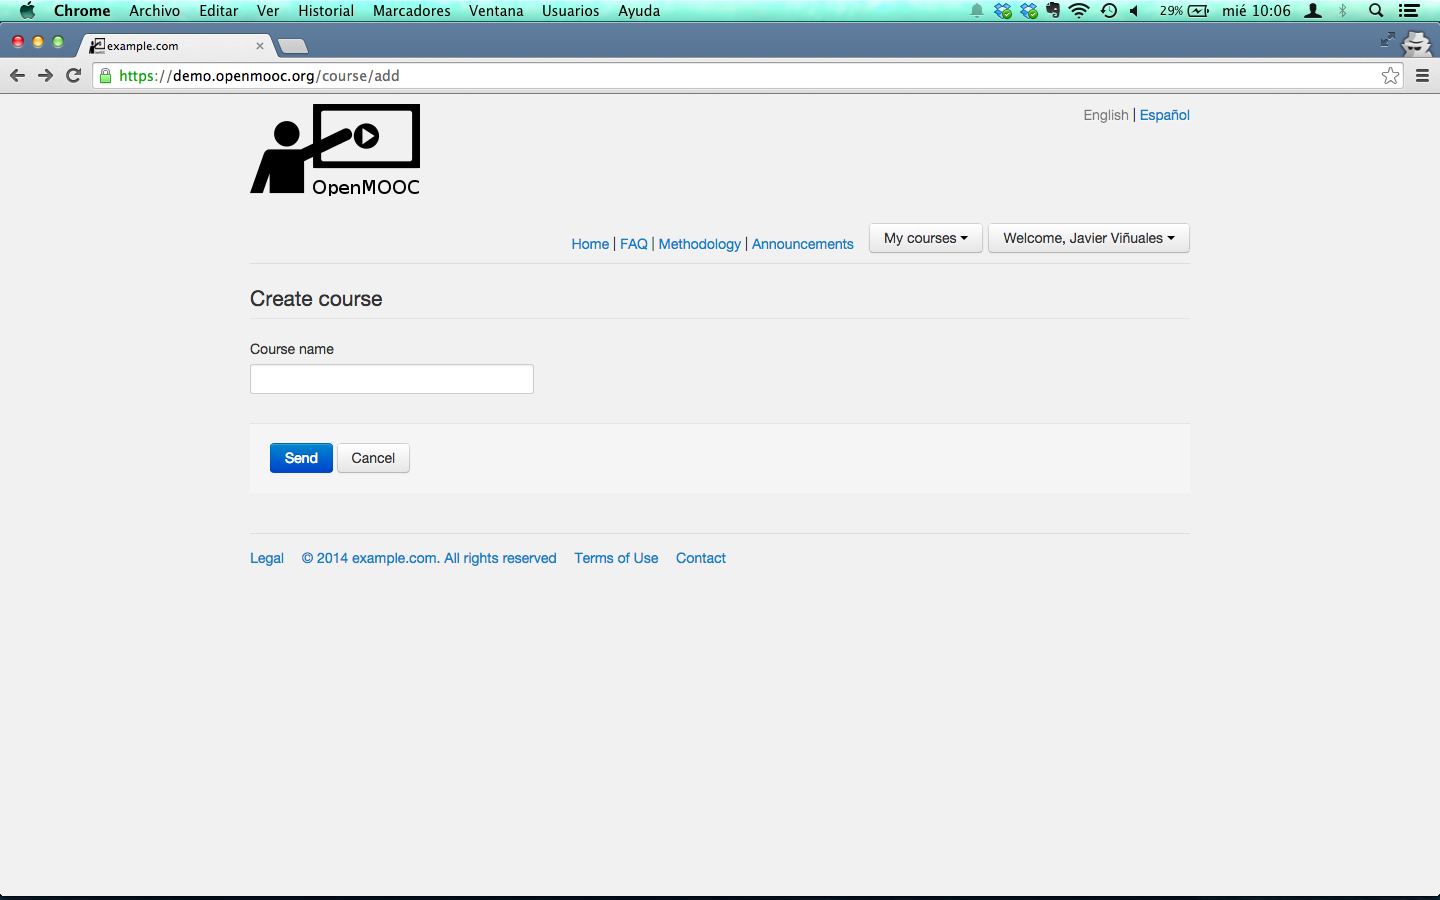
\includegraphics{2_create_course-2.png}

The value in the \textbf{Display Name} field identifies the discussion in the
course content. The values in the \textbf{Category} and \textbf{Subcategory} fields
appear in the list of discussion topics on the \textbf{Discussion} page. To
uniquely identify the discussion in your course, each \textbf{Category} /
\textbf{Subcategory} pair that you supply must be unique.

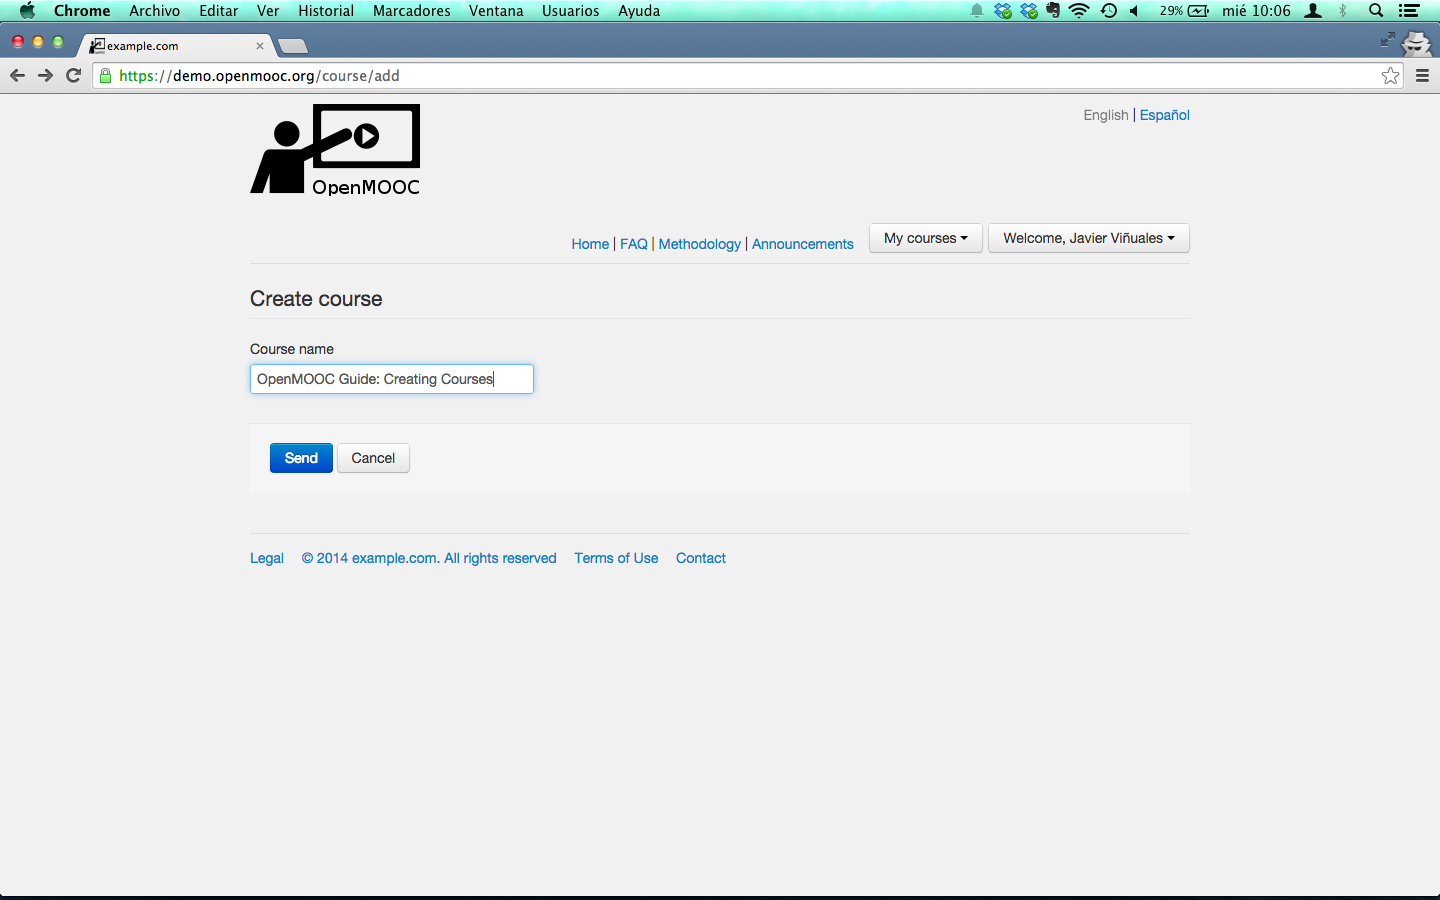
\includegraphics{3_create_course-3.png}

\end{enumerate}


\chapter{Course index}
\label{course_index:course-index}\label{course_index::doc}\label{course_index:id1}

\section{Overview}
\label{course_index:overview}
You can add a Discussion component to a unit, to pose a question related to the
Unit and give students a chance to respond and interact.


\section{Create a Discussion Component}
\label{course_index:create-a-discussion-component}\begin{enumerate}
\item {} 
Under \textbf{Add New Component}, click \textbf{Discussion}.

\item {} 
In the Discussion component that appears, click \textbf{Edit}.

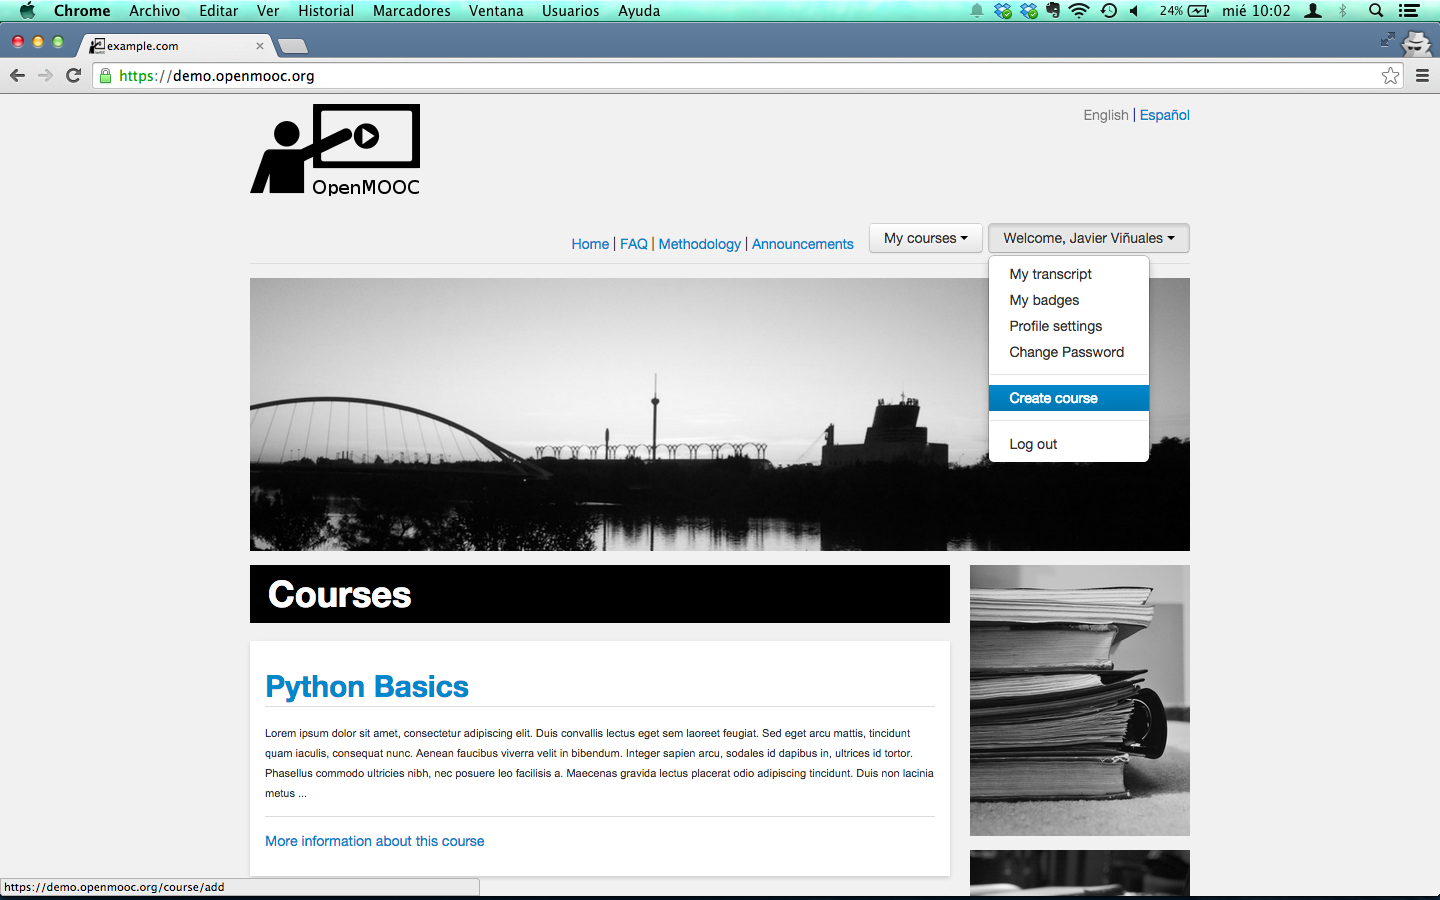
\includegraphics{1_create_course-1.png}

\item {} 
When the Discussion component editor opens, follow the guidelines in the
editor to fill in the \textbf{Category}, the optional \textbf{Display Name}, and the
\textbf{Subcategory} fields.

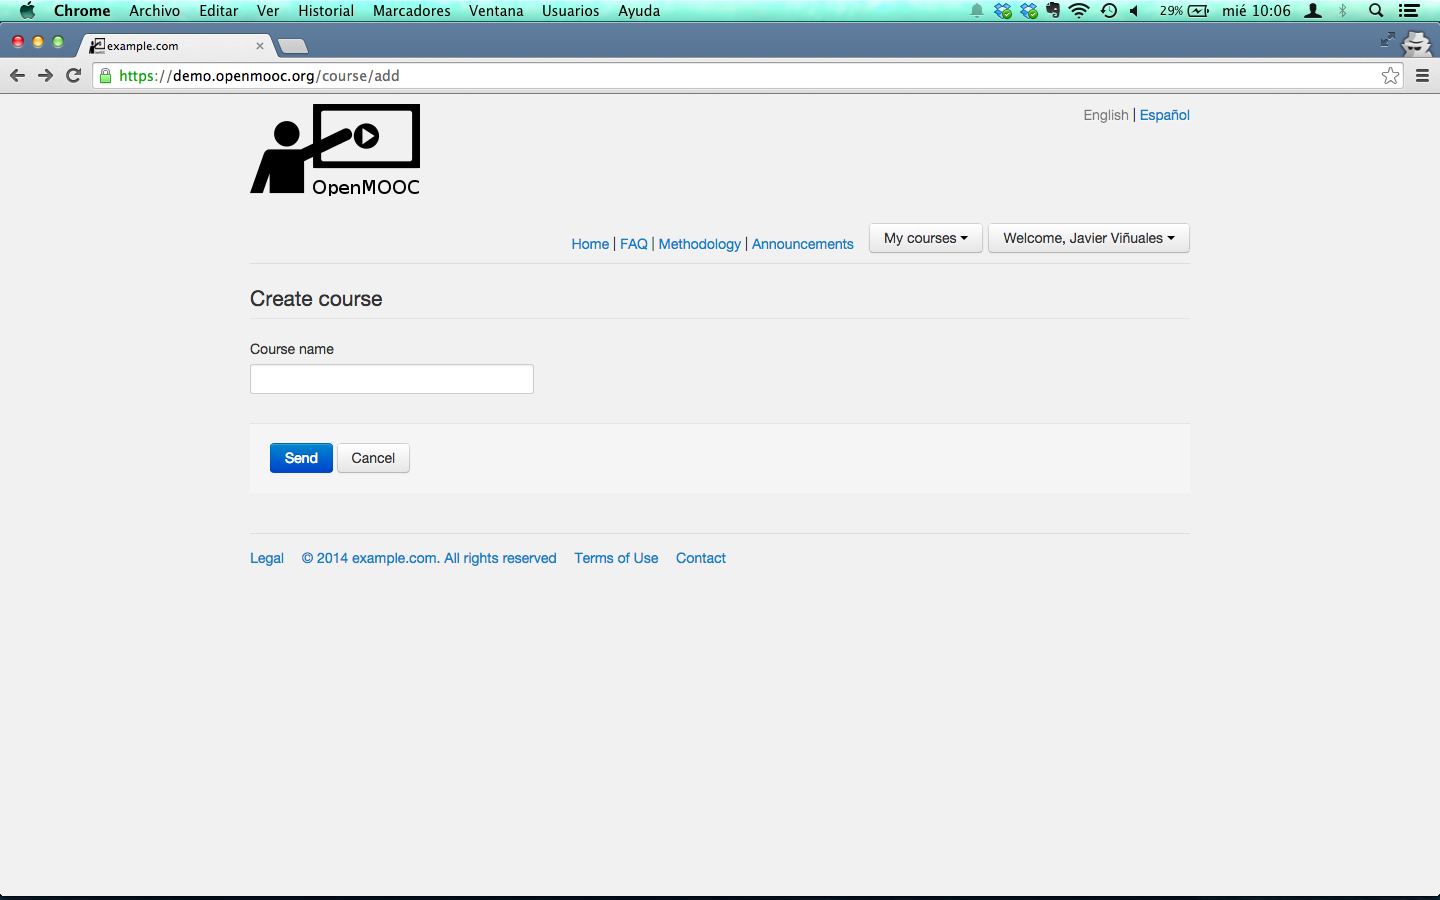
\includegraphics{2_create_course-2.png}

The value in the \textbf{Display Name} field identifies the discussion in the
course content. The values in the \textbf{Category} and \textbf{Subcategory} fields
appear in the list of discussion topics on the \textbf{Discussion} page. To
uniquely identify the discussion in your course, each \textbf{Category} /
\textbf{Subcategory} pair that you supply must be unique.

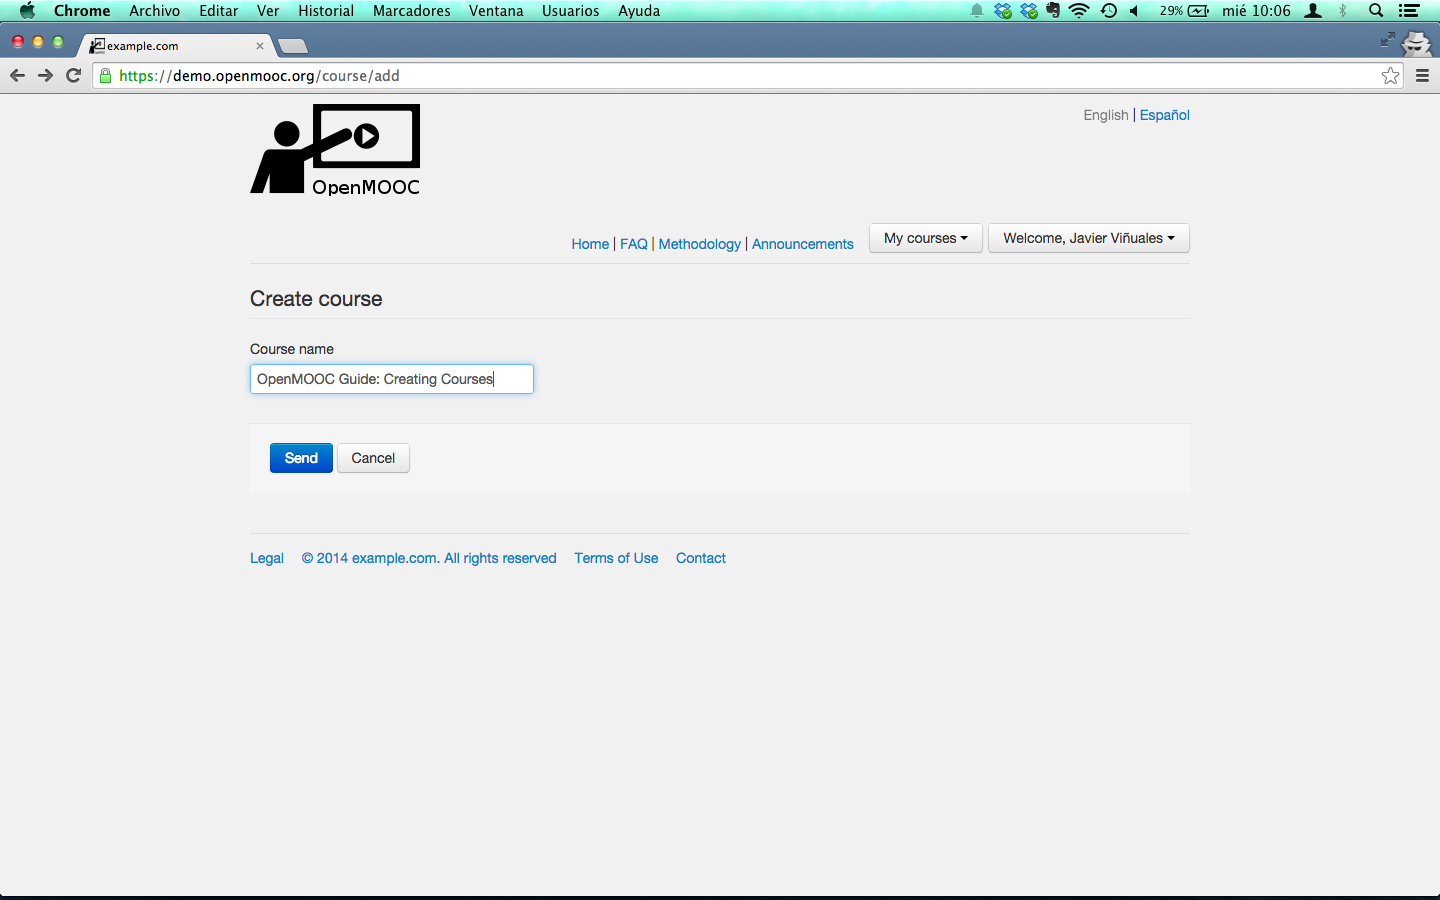
\includegraphics{3_create_course-3.png}

\end{enumerate}


\chapter{Course view}
\label{course_view:course-view}\label{course_view::doc}\label{course_view:id1}

\section{Overview}
\label{course_view:overview}
You can add a Discussion component to a unit, to pose a question related to the
Unit and give students a chance to respond and interact.


\section{Create a Discussion Component}
\label{course_view:create-a-discussion-component}\begin{enumerate}
\item {} 
Under \textbf{Add New Component}, click \textbf{Discussion}.

\item {} 
In the Discussion component that appears, click \textbf{Edit}.

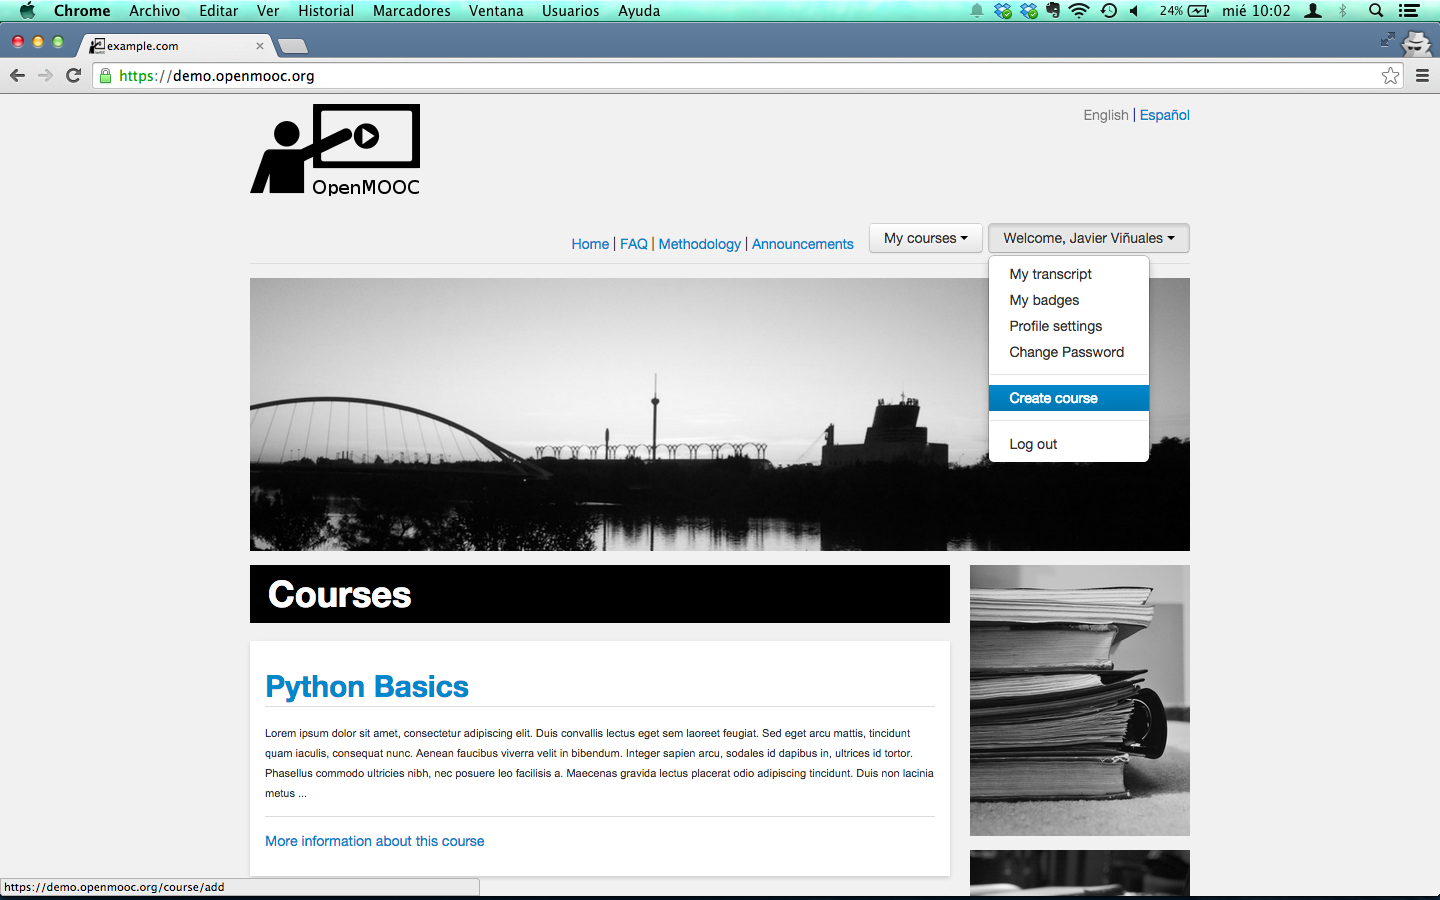
\includegraphics{1_create_course-1.png}

\item {} 
When the Discussion component editor opens, follow the guidelines in the
editor to fill in the \textbf{Category}, the optional \textbf{Display Name}, and the
\textbf{Subcategory} fields.

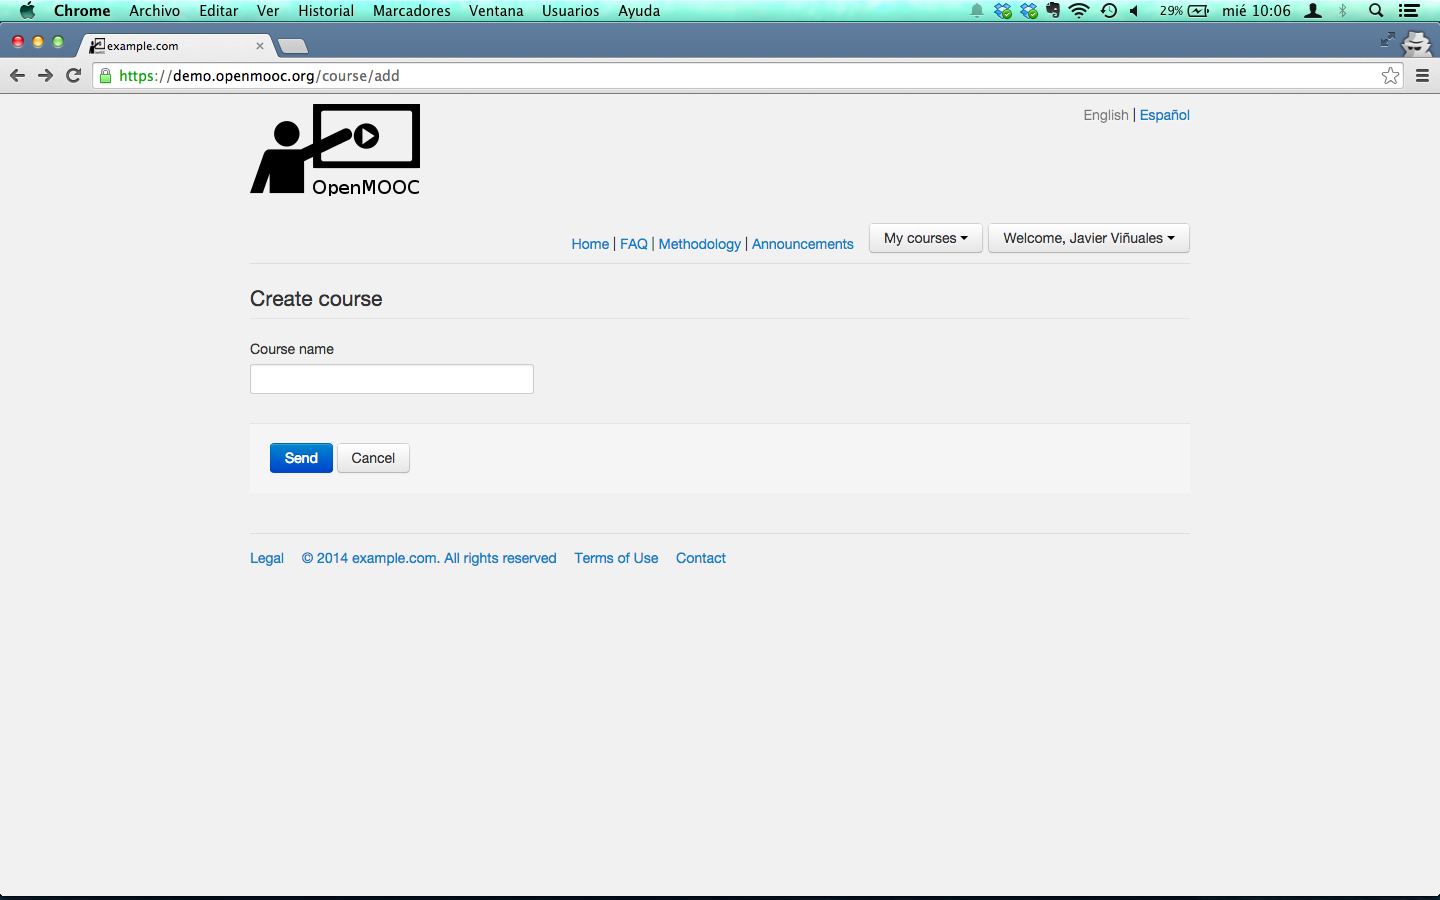
\includegraphics{2_create_course-2.png}

The value in the \textbf{Display Name} field identifies the discussion in the
course content. The values in the \textbf{Category} and \textbf{Subcategory} fields
appear in the list of discussion topics on the \textbf{Discussion} page. To
uniquely identify the discussion in your course, each \textbf{Category} /
\textbf{Subcategory} pair that you supply must be unique.

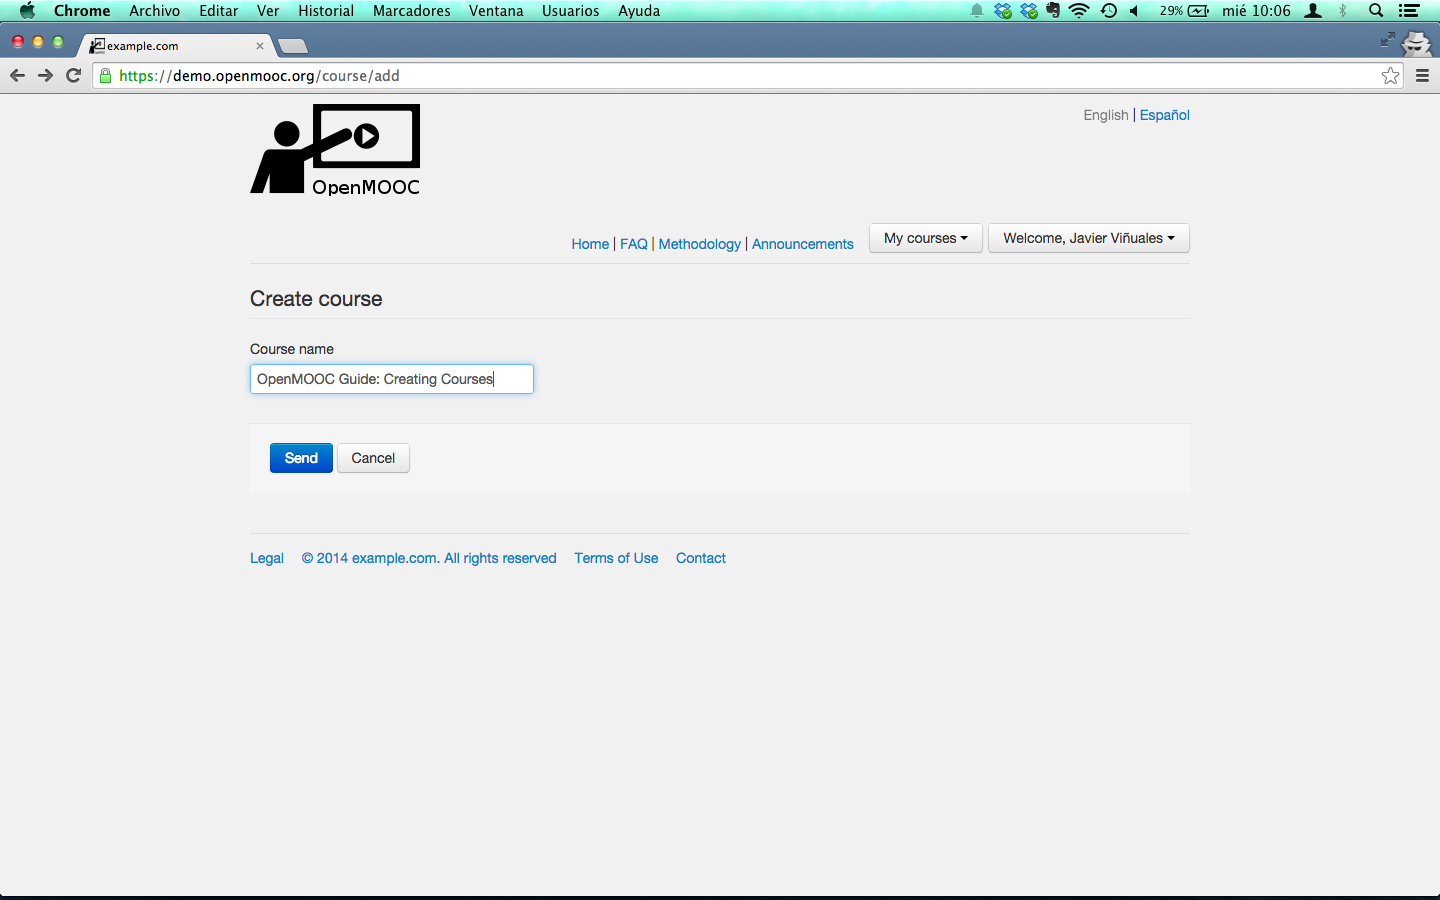
\includegraphics{3_create_course-3.png}

\end{enumerate}


\chapter{Pill view}
\label{pill_view:pill-view}\label{pill_view::doc}\label{pill_view:id1}

\section{Overview}
\label{pill_view:overview}
You can add a Discussion component to a unit, to pose a question related to the
Unit and give students a chance to respond and interact.


\section{Create a Discussion Component}
\label{pill_view:create-a-discussion-component}\begin{enumerate}
\item {} 
Under \textbf{Add New Component}, click \textbf{Discussion}.

\item {} 
In the Discussion component that appears, click \textbf{Edit}.

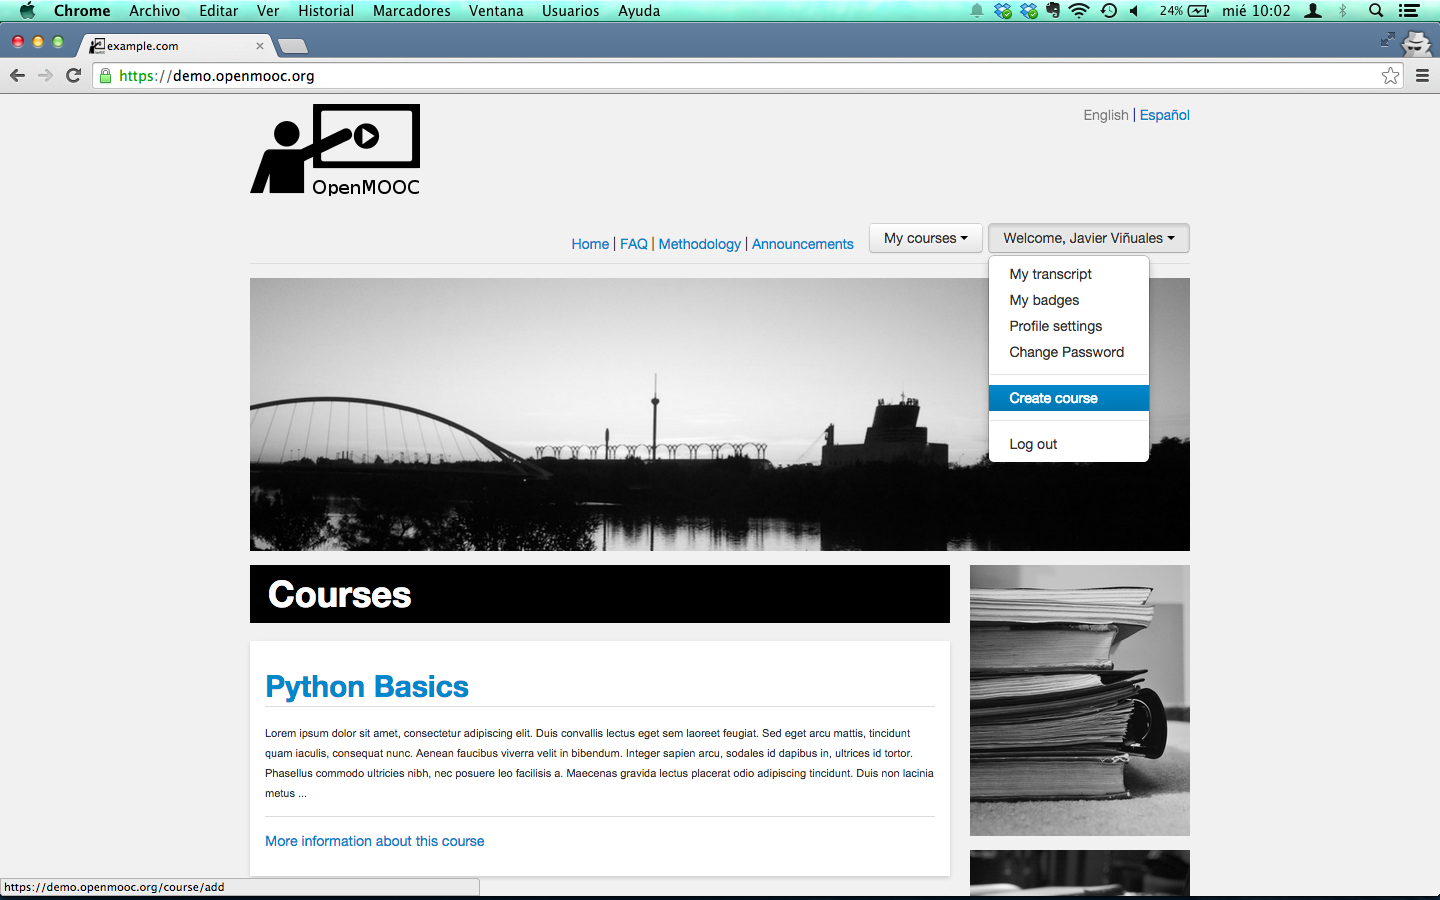
\includegraphics{1_create_course-1.png}

\item {} 
When the Discussion component editor opens, follow the guidelines in the
editor to fill in the \textbf{Category}, the optional \textbf{Display Name}, and the
\textbf{Subcategory} fields.

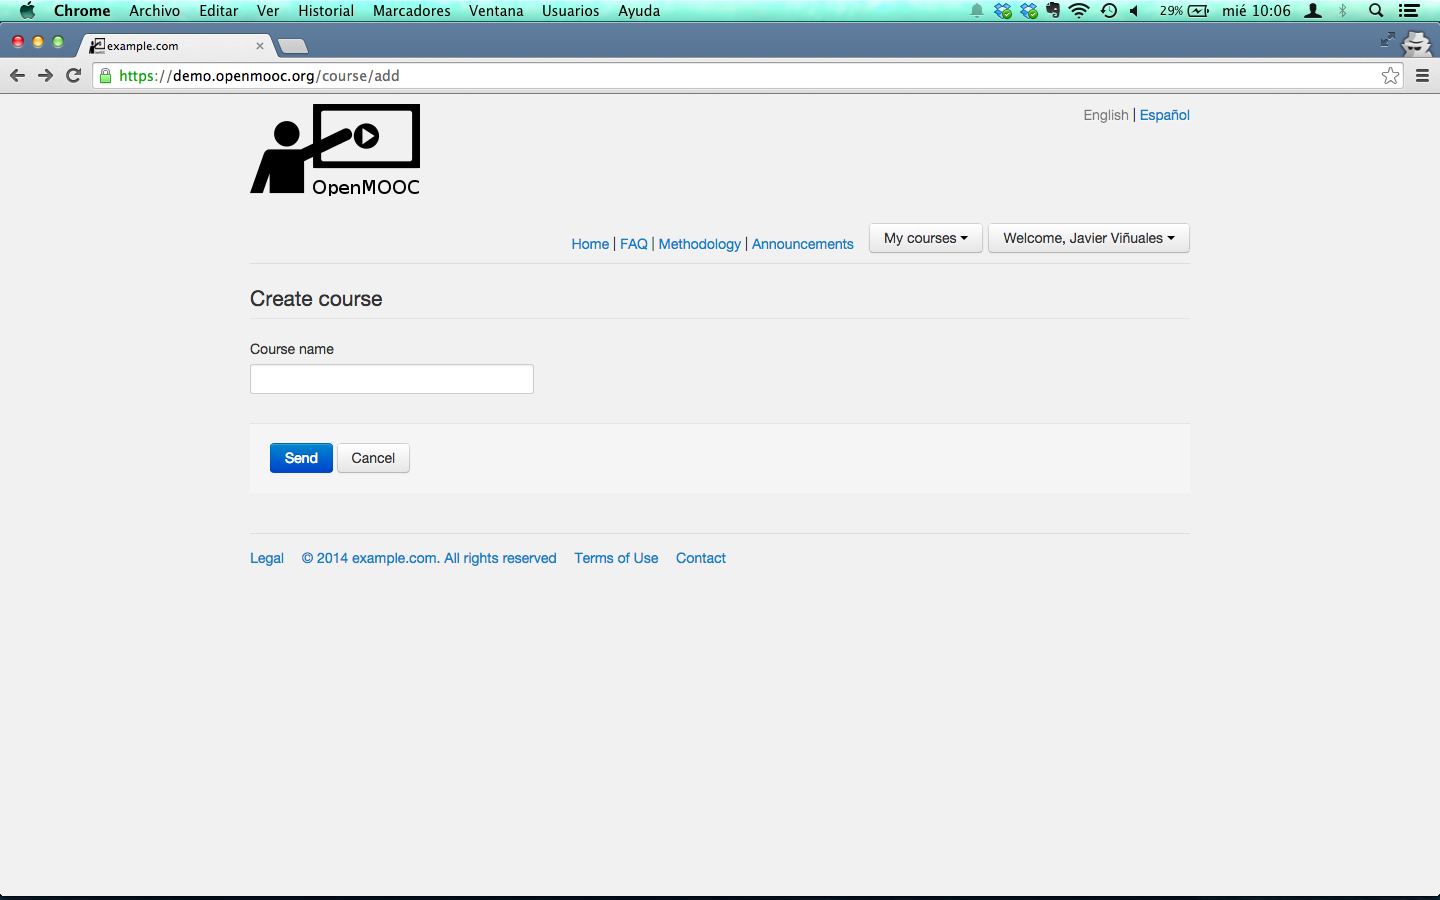
\includegraphics{2_create_course-2.png}

The value in the \textbf{Display Name} field identifies the discussion in the
course content. The values in the \textbf{Category} and \textbf{Subcategory} fields
appear in the list of discussion topics on the \textbf{Discussion} page. To
uniquely identify the discussion in your course, each \textbf{Category} /
\textbf{Subcategory} pair that you supply must be unique.

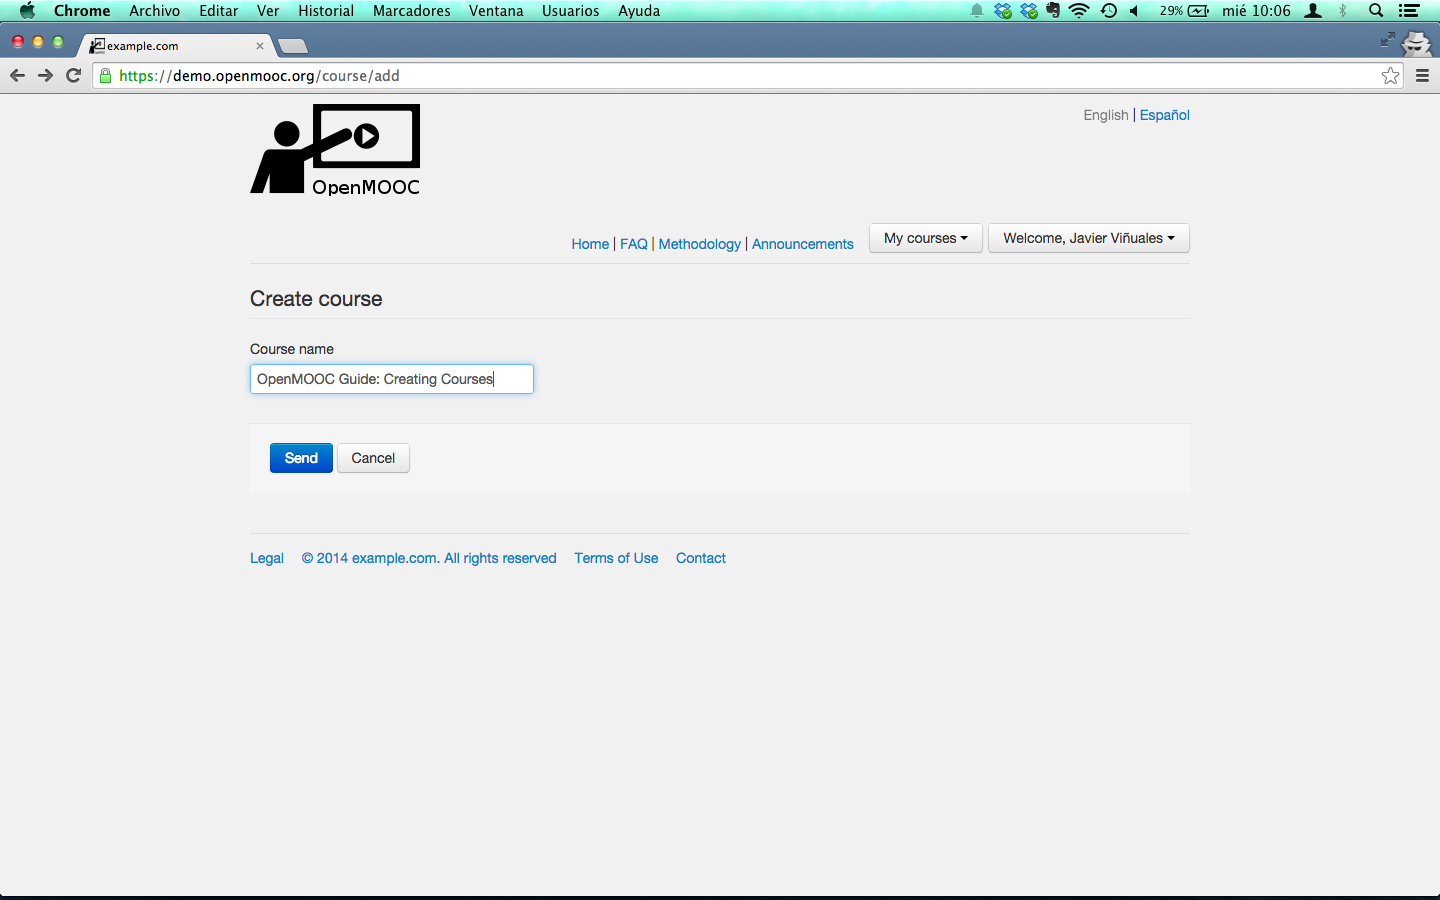
\includegraphics{3_create_course-3.png}

\end{enumerate}



\renewcommand{\indexname}{Index}
\printindex
\end{document}
